% !Mode:: "TeX:DE:UTF-8:Main"
\PassOptionsToPackage{check-declarations,enable-debug}{expl3}

% Note on the compilation of the documentation:
% The documentation uses for the tagging sometimes code 
% that is under development and/or not public yet. 
% To compile an *untagged* documentation, comment the line with
% the testphase keys in the following \DocumentMetadata command. 

\DocumentMetadata
 {
   % comment the following line to compile an untagged documentation:
   testphase=phase-III,
   pdfversion=2.0,lang=en-UK,pdfstandard=a-4,
   %uncompress
 }
\DebugBlocksOff
\makeatletter
\def\UlrikeFischer@package@version{0.98m}
\def\UlrikeFischer@package@date{2023-10-23}
\makeatother

\documentclass[bibliography=totoc,a4paper]{article}
\usepackage{geometry}
\usepackage[english]{babel}

\usepackage{unicode-math}
\setmainfont{Heuristica}
\usepackage[nopatch]{microtype}


\usepackage[autostyle]{csquotes}
\usepackage[style=numeric]{biblatex}
\addbibresource{tagpdf.bib}

\usepackage[noparboxrestore]{marginnote}
\makeatletter 
\renewcommand*{\mn@parboxrestore}{\tagpdfparaOff}%
\makeatother
\reversemarginpar

\usepackage{tcolorbox}
%think later ...

\usepackage{tikz}
\usetikzlibrary{positioning}
\usetikzlibrary{fit,tikzmark}
\usetikzlibrary{arrows.meta}
\tikzset{arg/.style = {font=\footnotesize\ttfamily, anchor=base,draw, rounded corners,node distance=2mm and 2mm}}
\tikzset{operator/.style = {font=\footnotesize\ttfamily, anchor=base,draw, rounded corners,node distance=4mm and 4mm}}


\usepackage{listings}
\lstset{basicstyle=\ttfamily, columns=fullflexible,language=[LaTeX]TeX,
        escapechar=*,
        commentstyle=\color{green!50!black}\bfseries}

% this allow to get real spaces in the code parts. 
% This should perhaps be combined in a new listings key
\lstset{showspaces}
\makeatletter \def\lst@visiblespace{\lst@ttfamily{\char32}{\char32}}\makeatother


\tagpdfsetup{
 tabsorder=structure,
 %log=v
 %show-spaces
 }

\usepackage[pdfdisplaydoctitle=true]{hyperref}

 \hypersetup{
  pdftitle={The tagpdf package, v\csname UlrikeFischer@package@version\endcsname},
  pdfauthor=Ulrike Fischer,
  colorlinks}

\tcbuselibrary{documentation}
%less space between docCommand
\tcbset{nosep/.style={doc raster command={raster after skip=-10pt}}}
\definecolor{Definition}{rgb}{0,0.2,0.6}
\newcommand\PrintKeyName[1]{\textsf{#1}}
\newcommand\pkg[1]{\texttt{#1}}
\newcommand\DescribeKey[1]{\texttt{#1}}
%\newcommand\cs[1]{\texttt{\textbackslash #1}}
%\usepackage{ydoc-desc} %hm hyperref ist ein Problem ...


\usepackage{tagpdfdocu-patches}

\newcommand\PDF{PDF}

\title{The \pkg{tagpdf} package, v\csname UlrikeFischer@package@version\endcsname}
\date{\csname UlrikeFischer@package@date\endcsname}
\author{Ulrike Fischer\thanks{fischer@troubleshooting-tex.de}}

\usepackage{shortvrb}
\MakeShortVerb|

\begin{document}

\tagstructbegin{tag=Title}
\begin{center}%
\let\thanks\footnote
\makeatletter
\huge \@title \par
\vskip .5em
\@author \par
\vskip 1em%
\@date \par
\end{center}%
\tagstructend





\tagstructbegin{tag=Div}
\begin{tcolorbox}[colframe=red,before upper=\tagpdfparaOn]

This package is not meant for normal document production. It is mainly a tool to \emph{research}
tagging.

You need a very current \LaTeX{} format.
You need a very current L3 programming layer.
You need the new \LaTeX{} PDF management bundle.

This package is incomplete, experimental and quite probably contains bugs. It is in parts
quite slow as the code prefers readability over speed.
At some time it will disappear when the code has been integrated into the \LaTeX{} format.

This package can change in an incompatible way.

You need some knowledge about \TeX, \PDF{} and perhaps even lua to use it.

\medskip

Issues, comments, suggestions should be added as issues to the github tracker:

\medskip
\centering
\url{https://github.com/u-fischer/tagpdf}

\end{tcolorbox}
\tagstructend


\tagtool{sec-add-grouping=false}

\tableofcontents

\tagtool{sec-add-grouping}


\section{Introduction}

Since many years the creation of accessible, tagged \PDF{}-files with \LaTeX\ which conform to the PDF/UA standard has been on the agenda of \TeX-meetings. Many people agree that this is important and Ross Moore has done quite some work on it. There is also a TUG-mailing list and a web page \parencite{tugaccess} dedicated to this theme.

In my opinion missing were means to \emph{experiment} with tagging and accessibility. Means to try out, how difficult it is to tag some structures, means to try out, how much tagging is really needed (standards and validators don't need to be right \ldots), means to test what else is needed so that a \PDF{} works e.g. with a screen reader, means to try out how core \LaTeX\ commands behave if tagging is used. Without such experiments it is in my opinion
quite difficult to get a feeling about what has to be done, which kernel changes are needed, how packages should be adapted.

This package was developed to close this gap by offering \emph{core} commands to tag a \PDF{}%
\footnote{In case you don't know what this means: there will be some explanations later on.}.
My hope was that the knowledge gained by the use of this package will at the end 
allow to decide if and how code to do tagging should be part of the \LaTeX\ kernel.


The code has been written so that it can be added as module to the \LaTeX{} kernel itself if it turns out to be usable. 
It therefore avoid to patch commands from other packages and is also not an aim of the package to develop such patches. While at the end changes to various commands in many classes and packages will be needed to get tagged \PDF{} files 
these changes should be done by the class, package and document writers themselves using a sensible API provided by the kernel and not by some external package that adds patches everywhere and would need constant maintenance -- one only need to look at packages like tex4ht or bidi or hyperref to see how difficult and sometimes fragile this is.

The package is now a part of the Tagged PDF project and triggered already various changes in the LaTeX kernel and the engines: There is a new PDF management,
the new para hooks allows to automatically tag paragraphs, after changes in the output routine
page breaks and header and footer are handled correctly, the engines support
now structure destinations. More changes are in the latex-lab bundle and can be loaded through testphase keys.

I'm sure that tagpdf still has bugs. Bugs reports, suggestions and comments can be added to the issue tracker on github. \url{https://github.com/u-fischer/tagpdf}.

Please also check the github site and latex-lab for new examples and improvements.

\subsection{Tagging and accessibility}

While the package is named \texttt{tagpdf} the goal is also \emph{accessible} \PDF{}-files. Tagging is \emph{one} (the most difficult) requirement for accessibility but there are others. I will mention some later on in this documentation, and -- if sensible -- I will also try to add code, keys or tips for them.

So the name of the package is a bit wrong. As excuse I can only say that it is shorter and easier to pronounce.


\subsection{Engines and modes}

The package works theoretically with all engines,
but the xelatex and the latex-dvips-route are basically untested tested and they also don't support
real space glyphs so I don't recommend them. 
lualatex is the most powerful and safe modus and should be used for new documents, it is slower than pdflatex but requires less compilations to get tagging. pdflatex works ok and can be used for legacy documents; it needs more compilations to resolve all cross references needed for the tagging. 

The package has two modes: the \emph{generic mode} which should work in 
theory with every engine and the \emph{lua mode} which works only with 
lualatex and (since version 0.98k) with dvilualatex. 

I implemented the generic mode first. Mostly because my \TeX\ skills are much better than my lua skills and I wanted to get the \TeX\ side right before starting to fight with attributes and node traversing.

While the generic mode is not bad and I spent quite some time to get it working I nevertheless think that the lua mode is the future and the only one that will be usable for larger documents. \PDF{} is a page orientated format and so the ability of luatex to manipulate pages and nodes after the \TeX-processing is really useful here. Also with luatex characters are normally already given as unicode.

The package uses quite a lot labels (in generic mode more than with luamode). At the begin it relied on the \pkg{zref} package, but switched now to a new experimental implementation for labels. The drawback of the new method is that they don't give yet good rerun messages if they have changed. I advise to use the \pkg{rerunfilecheck} package as a intermediate work-around and when using pdflatex compile
at best at least once or twice more often then normal.


\subsection{References and target PDF version}

My main reference for the first versions of this package was the free 
reference for \PDF{} 1.7. \parencite{pdfreference} and so the first versions 
of the package implemented only \PDF{} 1.7. 

In 2018 \PDF{} 2.0. has been released. The reference can be bought at no cost 
through the PDF association. 

\PDF{} 2.0 has a number of features that are really needed for good tagging: 
it knows more structure types, it allows to add associated files to 
structures---these are small, embedded files which can for example contain 
the mathML or source code of an equation---, it knows structure destinations 
which allows to link to a structure. 


\PDF{}~2.0 features are currently (mid 2023) not well supported by 
\PDF~consumer. No PDF viewer (including Acrobat) for example can handle name 
spaces and associated files. PAC~3 even crashes if one tries to load a \PDF{} 
2.0 file, and pdftk will create a \PDF{}~1.0 from it. 

Nevertheless \LaTeX{} targets \PDF{} 2.0, tagpdf has added support for 
associated files, for name spaces and other \PDF{} 2.0 features tagpdf and we 
recommend to use \PDF{} 2.0 if possible and then to complain to the PDF{} 
consumer if something doesn't work.   

The package doesn't try to suppress all 2.0 features if an older \PDF{} 
version is produced. It normally doesn't harm if a \PDF{} contains keys 
unknown in its version and it makes the code faster and easier to maintain if 
there aren't too many tests and code pathes; so for example associated files 
will always be added. But tests could be added in case this leads to 
incompabilities. 


\subsection{Validation}


\PDF{}'s created with the commands of this package must be validated:

\begin{itemize}
\item
 One must check that the \PDF{} is \emph{syntactically} correct. 
 It is rather easy to create broken \PDF{}:
 e.g. if a chunk is opened on one page but closed 
 on the next page or if the document isn't compiled often enough.

\item One must check how good the requirements of the PDF/UA standard are 
    followed \emph{formally}\footnote{The PDF/UA-2 standard for \PDF~2.0 
    will hopefully be released in 2023}. 

\item
One must check how good the accessibility is \emph{practically}.
\end{itemize}


Syntax validation and formal standard validation can be done with preflight 
of the (non-free) adobe acrobat. It can also be done also with the free 
\PDF{} Accessibility Checker (PAC~2021) \parencite{pac3}. There is also the 
validator veraPDF \parencite{verapdf}. A rather new and quite useful tool is 
\enquote{Next Generation PDF} \parencite{ngpdf}, a browser application which 
converts a tagged PDF to html, allows to inspect its structure and also to 
edit the structure. 

Practical validation is naturally the more complicated part. 
It needs screen reader, users which actually knows how to handle them, 
can test documents and can report where a \PDF{} has real accessibility problems.


\minisec{Preflight woes}

Sadly validators can not be always trusted. 
As an example for an reason that I don't understand the adobe preflight 
don't like the list structure \texttt{L}.
It is also possible that validators contradict: that the one says everything is okay, 
while the other complains.



\subsection{Examples wanted!}


To make the package usable examples are needed: 
examples that demonstrate how various structures can be tagged and which patches are needed, 
examples for the test suite, examples that demonstrates problems.


\begin{tcolorbox}
Feedback, contribuations and corrections are welcome!
\end{tcolorbox}


All examples should use the \cs{DocumentMetadata} key \PrintKeyName{uncompress}
so that uncompressed \PDF{} are created and the internal objects and 
structures can be inspected and be compared by the l3build checks.%


\section{Changes}

This section lists only important changes. More can be found in the \texttt{CHANGELOG.MD} and by checking the git commits.

\subsection{Changes in 0.3}


In this version I improved the handling of alternative and actual text. See section~\ref{sec:alt}. This change meant that the package relies on the module \texttt{l3str-convert}.

I no longer try to (pdf-)escape the tag names: it is a bit unclear how to do it at best with luatex. This will perhaps later change again.


\subsection{Changes in 0.5}


I added code to handle attributes and attribute classes, see section~\ref{sec:attributes} and corrected a small number of code errors.

I added code to add \enquote{real} space glyphs to the \PDF{}, see section \ref{sec:spacechars}.



\subsection{Changes in 0.6}


\textbf{Breaking change!} The attributes used in luamode to mark the MC-chunks are no longer set globally. I thought that global attributes would make it easier to tag, but it only leads to problem when e.g. header and footer are inserted. So from this version on the attributes are set locally and the effect of a \verb+\tagmcbegin+ ends with the current group. This means that in some cases more \verb+\tagmcbegin+ are needed and  this affected some of the examples, e.g. the patching commands for sections with KOMA. On the other side it means that quite often one can omit the \verb+\tagmcend+ command.


\subsection{Changes in version 0.61}

\begin{itemize}
\item internal code adaptions to expl3 changes.
\item dropped the compresslevel key  -- probably not needed.
\end{itemize}


\subsection{Changes in version 0.8}

\begin{itemize}
\item  As a first step to include the code proper in the \LaTeX\ kernel the module name has changed from \texttt{uftag} to \texttt{tag}. The commands starting with |\uftag| will stay valid for some time but then be deprecated.

\item \textbf{Breaking change!} The argument of \texttt{newattribute} option should no longer add the dictionary bracket \verb+<<..>>+, they are added by the code.


\item \textbf{Breaking change!} The package now requires the new PDF management as provided for now by the package \pkg{pdfmanagement-testphase}. \pkg{pdfmanagement-testphase},
prepares the ground for better support for tagged PDF in \LaTeX{}.
It is part of a larger project to automatically generate tagged PDF \url{https://www.latex-project.org/news/2020/11/30/tagged-pdf-FS-study/}

\item Support to add associated files to structures has been added with new keys \texttt{AF}, \texttt{AFinline} and \texttt{AFinline-o}.

\item \textbf{Breaking change!} The support for other 8-bit input encodings has been removed.
utf8 is now the required encoding.

\item The keys |lang|, |ref| and |E| have been added for structures.

\item The new hooks of LaTeX are used to tagged many paragraphs automatically. The small red numbers around paragraphs in the documentation show them in action. The main problem here is not to tag a paragraph, but to avoid to tag too many: paragraphs pop up in many places.
\end{itemize}

\subsection{Changes in version 0.81}

\begin{itemize}
\item Hook code to tag links (URI and GoTo type) have been added. So normally they should simply work if tagging
is activated.

\item Commands and keys to allow automatic paragraph tagging have been added. See section~\ref{sec:paratagging}.
As can be seen in this documentation the code works quite good already, but one should be aware that \enquote{paragraphs} can appear in many places and sometimes there are even more paragraph begin than ends.

\item A key to test if local or global setting of the mc-attributes in luamode is more sensible, see \ref{sec:global-local} for more details.

\item New commands to store and reset mc-tags.

\item PDF 2.0 namespaces are now supported.
\end{itemize}

\subsection{Changes in version 0.82}

A command |\tag_if_active:TF| to test if tagging is active has been added. This allow external packages to write conditional code.

The commands |\tag_struct_parent_int:| and |\tag_struct_insert_annot:nn| have been added. They allow to
add annotations to the structure.


\subsection{Changes in version 0.83}

|\tag_finish_structure:| has been removed, it is no longer a public command.

\subsection{Changes in version 0.90}

\begin{itemize}
\item Code has been cleaned up and better documented.

\item \textbf{More engines supported} The generic mode of \pkg{tagpdf} now works
(theoretically, it is not much tested) with all engines supported
by the \PDF\ management. 
So compilations with Xe\LaTeX{} or with dvips should work. But it should be noted that
these engines and backends don't support the |interspaceword| option. With Xe\LaTeX{} it is perhaps possible
implement something with |\XeTeXinterchartoks|, but for the dvips route I don't see an option (apart from lots
of manual macros everywhere).
\item \textbf{MC-attributes are global again} In\sidenote{Breaking change!} version 0.6 the attributes used in
luamode to mark the MC-chunks were no longer set globally. This avoided a number of problems with header and footer
and background material, but further tests showed that it makes it difficult to correctly mark things like
links which have to interrupt the current marking code---the attributes couldn't easily escape groups added by
users. See section~\ref{sec:global-local} for more details.
\item \textbf{key global-mc removed:} Due to the changes in the attribute keys this key is not longer needed.
\item \textbf{key check-tags removed:} It doesn't fit. Checks are handled over the logging level.
\item |\tagpdfget| has been removed, use the expl3 version if needed.
\item The show commands |\showtagpdfmcdata|, |\showtagpdfattributes|, |\showtagstack| have been removed and replaced
by a more flexible command |\ShowTagging|.
\item The commands |\tagmcbegin| and |\tagmcend| no longer ignore following spaces or remove earlier one. While this
is nice in some places, it also ate spaces in places where this wasn't expected. From now on both commands behave exactly
like the expl3 versions.
\item The lua-code to add real space glyphs has been separated from the tagging code. This means that |interwordspace| now
works also if tagging is not active.
\item The key |activate| has been added, it open the first structure, see below.
\end{itemize}

\subsection{Changes in version 0.92}

\begin{itemize}
\item support for page breaks in pdftex has been added, see  section~\ref{sec:splitpara},


\item header and footer are tagged as artifacts automatically, see section~\ref{sec:header-footer}.

\item keys \texttt{alttext-o} and \texttt{actualtext-o} has been removed. \texttt{alttext} and \texttt{actualtext}
will now expand once.

\end{itemize}




\subsection{Changes in version 0.93}

\begin{itemize}
\item Support for associated files in the root element (key \texttt{root-AF})
has been added. This allow e.g. to add a css-file which is be used if the \PDF\ is converted to
html.

\item First steps have been done to adapt the package to planed changes in \LaTeX{}:
The command \cs{DocumentMetadata} will be
added to the format and will take over the role of \cs{DeclareDocumentMetadata}
from \pkg{pdfmanagement-testphase} and additionally
will also load the pdf management code. This will simplify the documents
as it will no longer be needed to load the package.

\item The package has now support for \enquote{structure destinations}.
This is a new type of destinations in \PDF~2.0.
For pdftex and luatex this requires new binaries. They will be included
in texlive 2022, miktex already has the new pdftex, the new luatex will probably follow soon.

\item The commands \cs{tagpdfifluatexT}, \cs{tagpdfifluatexTF} has been removed \cs{tagpdfifpdftexT},

\end{itemize}

\subsection{Changes in version 0.94}

In this version a small package, \pkg{tagpdf-base} has been added. It provides
no-op versions of the main expl3 user commands for packages that want to support
tagging but can't be sure if the \pkg{tagpdf} package has been loaded.

\subsection{Changes in version 0.95}

Small bug fixes.

\subsection{Changes in version 0.96}

\begin{itemize}
\item The \texttt{alttext} key has been renamed to \texttt{alt}, the other key name exists as alias.

\item The new command |\tag_struct_object_ref:n| allows to
   create the object reference of a structure.

\item a new key \texttt{parent} has been added
   to allow structures to choose their parent structure.

\item a new option \texttt{paratag} allows to change the tag name used for the
   automatically tagged paragraphs.

\item the commands |\tag_start:|, |\tag_stop:|, |\tag_stop:n| and |\tag_start:n| allow
    to stop and start tagging (for example in trial typesetting).

\item Small bug fixes.
\end{itemize}

\subsection{Changes in version 0.98}

\begin{itemize}
\item The declarations of tag namespaces have been externalized and are now
read from files when \pkg{tagpdf} is loaded. 

\item The \PDF{} format (and some of the standards) declare various parent-child rules for
structure tags. A first step to implement this rules and check if they are fullfilled have
been done. More information can be found in section~\ref{sec:parent-child}.

\item As a side effect of the new rule checking, the requirements for new tags
 have been tightened: Adding a new tag with add-new-tag now requires that the target role is 
    defined. Unknown roles error. 
    
\item |\tagmcbegin| no longer requires that a tag is set, instead if will pick up
the tag name from the surrounding structure. 

\item Structure destination are now created also with \PDF \textless\,2.0. They shouldn't harm and
can improve the html export.

\end{itemize}

\subsection{Changes in version 0.98a}
Small bug fixes in code and documentation.

\subsection{Changes in version 0.98b}
The main change is from now on every structure has an ID and an IDtree is 
added. The ID of a structure can be retrieved with |\tag_get:n| 
see~\ref{sec:retrieve}. 


\subsection{Changes in version 0.98e}

\begin{itemize}
\item The main change is that the automatic paratagging uses now a two-level structure. This accompanies development
in the LaTeX github inthe \texttt{latex-lab} package regarding the tagging of blocks like lists or verbatim.
See~\ref{sec:paratagging} and also \texttt{latex-lab-block-tagging.dtx} for more background.

\item The command |tag_struct_end:n| has been add to improve debugging.
\end{itemize}

\subsection{Changes in version 0.98k}

The luamode has been adapted and now allows also the compilation with 
dvilualatex. By default it will insert specials for \texttt{dvips} into the 
dvi. But be aware that \texttt{dvips} can normally not be used as it can't 
handle open type fonts, and extended version would be needed which isn't in 
texlive yet. It is also possible to use \texttt{dvipdfmx} as backend (which 
already has support for open type fonts), for this you need to use 
\texttt{backend=dvipdfmx} in the \cs{DocumentMetadata} command. Real space 
chars will work, but are currently not taken from the current font. This will 
be improved in the next luaotfload version. The compilation with dvilualatex 
is not much tested yet. 

\subsection{Changes in version 0.98l}

In 2023 the primitives to write literal code into the pdf have been extended in all engines
and now allow to delay the expansion of their argument to the shipout. This made it possible to greatly simplify and speed up the code used in generic mode to number the MC-chunks. In most cases building the structure should now need only two or three compilations. The new code requires a current pdfmanagement-testphase and is then used automatically if the new engines are detected. 

\subsection{Proof of concept: the tagging of the documentation itself}

Starting with version 0.6 the documentation itself has been tagged. The 
tagging wasn't (and isn't) in no way perfect. The validator from Adobe didn't 
complain, but PAC~3 wanted alternative text for all links (no idea why) and 
so I put everywhere simple text like \enquote{link} and \enquote{ref}. The 
links to footnotes gave warnings, so I disabled them. I used types from the 
\PDF{} version 1.7, mostly as I had no idea what should be used for code in 
2.0. Margin notes were simply wrong \ldots 

The tagging has been improved and automated over time in sync with 
improvements and new features in the LaTeX kernel and the \PDF\ management 
code and is now much better. Sadly the output of the validators don't quite 
reflect the improvements. The documentation uses now \PDF~2.0  and PAC~3 
can't handle this, it claims that the file is damaged. The Adobe validator 
has a bug and doesn't like the (valid) use of  the \texttt{Lbl} tag for the 
section numbers (see figure~\ref{fig:adobe}).  



But even if the documentation passed the tests of the validators:  as mentioned above passing a formal test doesn't mean that the content is really good and usable. I have a lot doubts that the code parts are really readable. The bibliography and the references must be improved. The user commands used for the tagging and also some of the patches used are still rather crude. So there is lot space for improvement.

\begin{tcolorbox}[before upper=\tagpdfparaOn]
Be aware that to create the tagged version a current lualatex-dev and a current version of the pdfmanagment-testphase package is needed.
\end{tcolorbox}


\includegraphics[alt=PAC 3 report]{pac3}


\begin{figure}

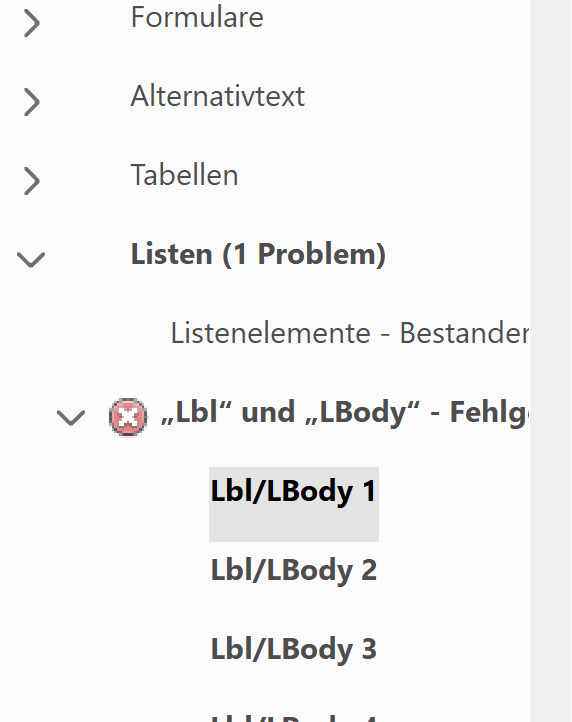
\includegraphics[alt={Screenshot of Adobe report}]{acrobat}

\caption{Adobe Acrobat complaining
about the \texttt{Lbl} use}\label{fig:adobe}\par

\end{figure}


\section{Loading}

The package requires the new PDF management. With a current \LaTeX{} (2022-06-01 or newer)
the PDF management is loaded if you use the \cs{DocumentMetadata} command before \cs{documentclass}.
The \texttt{tagpdf} package can then be loaded and activated by using the \texttt{testphase} key. The exact behaviour of
the \texttt{testphase} key is documented in \texttt{documentmetadata-support-doc.pdf} which
is part of the \texttt{latex-lab} bundle.

Various parts of the code differentiate between \PDF{} version 2.0 and lower versions. If 
\PDF{} 2.0 is wanted it is required to set the version early in the \cs{DocumentMetadata}
command so that \pkg{tagpdf} can pick up the correct code path. 

\begin{taglstlisting}
\DocumentMetadata
 {
  % testphase = phase-I, % tagging without paragraph tagging
  testphase = phase-II % tagging with paragraph tagging and other new stuff.
  % testphase = phase-III % tagging with paragraph sec, toc, block tagging and more
  % pdfversion = 2.0   % pdfversion must be set here.
 }
\documentclass{article}
\begin{document}
some text
\end{document}
\end{taglstlisting}

\minisec{Deactivation}

When loading \pkg{tagpdf} through the \texttt{testphase} keys, it is automatically activated. 
To deactivate it while still retaining all the other new code from the latex-lab testphase files,
use in the preamble |\tagpdfsetup{activate-all=false}|. You can additionally also deactivate the 
paratagging and the interword space code. 
To suppress the loading of the package alltogether you can try

\begin{taglstlisting}
\makeatletter 
\disable@package@load{tagpdf}{}
\makeatother
\DocumentMetadata{...}
\end{taglstlisting}


\minisec{Loading as package needs activation!}

It is not recommended anymore, but the package can also be loaded normally with |\usepackage| 
(but it is
still required to use \cs{DocumentMetadata} to load the \PDF\ management) but
it will then -- apart from loading more packages and defining a lot of things -- not do much. You will have to \emph{activate} it with \verb+\tagpdfsetup+.

The \PDF\ management loaded with \cs{DocumentMetadata} will in any case load \texttt{tagpdf-base} a
small package that provides no-op versions of the main tagging commands.

Most commands do nothing if tagging is not activated, but in case a test is needed a command (with the usual p,T,F variants) is provided:

\begin{docCommand}{tag_if_active:TF}{}\end{docCommand}

The check is true only if \emph{everything} is activated. In all other cases (including if tagging has been stopped locally) it will be false.

\subsection{Modes and package options}


%TODO think about tagging of the keys. Aside? Header?


The package has two different modes: The \textbf{generic mode} works (in theory, currently only fully tested with pdflatex) probably with all engines, the \textbf{lua mode} only with lualatex. The differences between both modes  will be described later. The mode can be set with package options:

\DescribeKey{luamode}

This is the default mode. It will use the generic mode if the document is processed with pdflatex and the lua mode with lualatex.

\DescribeKey{genericmode}

This will force the generic mode for all engines.


\subsection{Setup and activation}\label{ssec:setup}


\begin{docCommand}{tagpdfsetup}{\marg{key-val-list}}\end{docCommand}

This command setups the general behaviour of the package.
The command should be normally used only in the preamble
(for a few keys it could also make sense to change them in the document).

The key-val list understands the following keys:

\begin{description}
\item[\PrintKeyName{activate-all}]
 Boolean, initially false. Activates everything, that's normally the sensible thing to do.
\item [\PrintKeyName{activate}] Like |activate-all|, \emph{additionally} is opens at begin document
a structure with |\tagstructbegin| and closes it at end document. The key accepts as value a tag name which is used as the tag of the structure.
The default value is |Document|.
\item[\PrintKeyName{activate-mc}]
 Boolean, initially false. Activates the code related to marked content.
\item[\PrintKeyName{activate-struct}]
 Boolean, initially false. Activates the code related to structures. Should be used only if \PrintKeyName{activate-mc} has been used too.
\item[\PrintKeyName{no-struct-dest}]
 Starting with version 0.93 \pkg{tagpdf} will create automatically structure destinations (see section~\ref{sec:struct-dest} if \pkg{hyperref} is used, if
 the engine supports it and if the pdf version is 2.0. With this key this can be suppressed.
\item[\PrintKeyName{activate-tree}]
Boolean, initially false. Activates the code related to trees. Should be used only if the two other keys has been used too.
\item[\PrintKeyName{add-new-tag}]
 Allows to define new tag names, see section \ref{sec:new-tag} for a description.
\item[\PrintKeyName{interwordspace}]
 Choice key, possible values are \PrintKeyName{true}/""\PrintKeyName{on} and \PrintKeyName{false}/\PrintKeyName{off}. The key activates/deactivates the insertion of space glyphs, see section~\ref{sec:spacechars}. In the luamode it only works if at least \PrintKeyName{activate-mc} has been used.

\item[\PrintKeyName{log}]
 Choice key, possible values \PrintKeyName{none}, \PrintKeyName{v}, \PrintKeyName{vv}, \PrintKeyName{vvv},  \PrintKeyName{all}.  Setups the log level.  Changing the value affects currently mostly the luamode: \enquote{higher} values gives more messages in the log. The current levels and messages have been setup in a quite ad-hoc manner and will need improvement.
\item[\PrintKeyName{newattribute}]
 This key takes two arguments and declares an attribute. See \ref{sec:attributes}.
\item[\PrintKeyName{show-spaces}]

Boolean.\sidenote{luamode}
That's a debug option, it helps in lua mode to see where space glyph will be inserted if \PrintKeyName{interwordspace} is activated.

\item[\PrintKeyName{paratagging}] Boolean. This activate/deactivates the automatic tagging of paragraphs, see 
 \ref{sec:paratagging} for more background.
 It uses the \texttt{para/begin} and \texttt{para/end} hooks of the newest \LaTeX{} version (2021-05-01).
 With more tagging support conditions will be added, that means the code is bound to change! Paragraphs can appear in many unexpected  places and the code can easily break, so there is also an option to see where such paragraphs are:

\item[\PrintKeyName{paratagging-show}] Boolean. This activate/deactivates small red and green numbers in the places where the paratagging hook code is used.

\item[\PrintKeyName{paratag}] String. This key changes the second tag used by the paratagging code. The default tag is \texttt{text}, a \LaTeX{} specific tag that is role mapped to \texttt{P}. A useful local setting here can be \texttt{NonStruct}, which creates a structure \enquote{without meaning}. For local changes it is recommended
    to use the newer \cs{tagtool} command described below instead of \cs{tagpdfsetup}.

\item[\PrintKeyName{tabsorder}]
 Choice key, possible values are \PrintKeyName{row}, \PrintKeyName{column}, \PrintKeyName{structure}, \PrintKeyName{none}.  This decides if a \verb+/Tabs+ value is written to the dictionary of the page objects. Not really needed for tagging itself, but one of the things you probably need for accessibility checks. So I added it. Currently the tabsorder is the same for all pages. Perhaps this should be changed \ldots.
\item[\PrintKeyName{tagunmarked}]
 Boolean,\sidenote{luamode} initially true. When this boolean is true, the lua code will try to mark everything that has not been marked yet as an artifact. The benefit is that one doesn't have to mark up every deco rule oneself. The danger is that it perhaps marks things that shouldn't be marked -- it hasn't been tested yet with complicated documents containing annotations etc. See also section~\ref{sec:lazy} for a discussion about automatic tagging.
\item[\PrintKeyName{uncompress}]
 Sets both the \PDF{} compresslevel and the \PDF{} objcompresslevel to 0 and so allows to inspect the \PDF{}.


\end{description}

\begin{docCommand}[nosep]{tagtool}{\marg{key-val}}\end{docCommand}
\begin{docCommand}{tag_tool:n}{\marg{key-val}}\end{docCommand}

The tagging of document elements require a variety of small commands. This command
will unify them under a common interface. This is work-in-progress and syntax and implementation
can change! While the argument looks like a key-val \emph{list} (and currently is actually one), 
this should not be relied on. Instead only
one argument should be used as the implementation will change to improve the speed. Currently the following 
arguments are supported

\begin{description}
\item[\PrintKeyName{para}] Boolean. It will replace the \cs{tagpdfparaOn} and \cs{tagpdfparaOff} command.
\item[\PrintKeyName{unittag}] String. It allows to change the outer tag used in the following automatically tagged paragraphs. The setting is local.
\item[\PrintKeyName{paratag}] String. It allows to change the inner tag used in the following automatically tagged paragraphs. The setting is local.
\item[\PrintKeyName{para-flattened}] Boolean. If set it will suppress the outer structure in the automatic paratagging. 
This should be applied to the start and end hook in the same way! The setting is local.

\end{description}



\section{Tagging}


pdf is a page orientated graphic format. It simply puts ink and glyphs at various coordinates on a page. A simple stream of a page can look like this\footnote{The appendix contains some remarks about the syntax of a \PDF{} file}:

\begin{taglstlisting}[columns=fixed]
stream
   BT
   /F27 14.3462 Tf                 %select font
   89.291 746.742 Td               %move point
   [(1)-574(Intro)-32(duction)]TJ  %print text
   /F24 10.9091 Tf                 %select font
    0 -24.35 Td                    %move point
    [(Let's)-331(start)]TJ         %print text
    205.635 -605.688 Td            %move point
    [(1)]TJ                        %print text
   ET
endstream
\end{taglstlisting}


From this stream one can extract the characters and their placement on the page 
but not their semantic meaning  (the first line is actually a section heading, 
the last the page number). And while in the example the order is correct 
there is actually no guaranty that the stream contains the text in the order 
it should be read.

Tagging means to enrich the \PDF{} with information about the \emph{semantic} 
meaning and the \emph{reading order}. (Tagging can do more, one can also 
store all sorts of layout information like font properties and indentation 
with tags. But as I already wrote this package concentrates on the part of 
tagging that is needed to improve accessibility.)


\subsection{Three tasks}


To tag a \PDF{} three tasks must be  carried out:

\begin{enumerate}
\item
 \textbf{The mark-content-task}:\sidenote{mc-task} The document must add 
 \enquote{labels} to the page stream which allows to identify and reference 
 the various chunks of text and other content.  
 This is the most difficult part of tagging -- both for the document writer 
 but also for the package code. At first there can be quite many 
 chunks as every one is a leaf node of the structure and so often a rather 
 small unit.  At second the chunks must be defined page-wise -- and 
 this is not easy when you don't know where the page breaks are. 
 Also in a standard document a lot text is created automatically, e.g. 
 the toc, references, citations, list numbers etc and it is not always 
 easy to mark them correctly.

\item \textbf{The structure-task}:\sidenote{struct-task}  The document must 
    declare the structure. This means marking the start and end of 
    semantically connected portions of the document (correctly nested as a 
    tree). This too means some work for the document writer, but less than 
    for the mc-task: at first quite often the mc-task and the 
    structure-task can be combined, e.g. when you mark up a list number or 
    a tabular cell or a section header; at second one doesn't have to worry 
    about page breaks so quite often one can patch standard environments to 
    declare the structure. On the other side a number of structures end in 
    \LaTeX\ only implicitly -- e.g. an item ends at the next item, so 
    getting the \PDF{} structure right still means that additional mark up 
    must be added. 


\item \textbf{The tree management}:\sidenote{tree-task} At last the 
    structure must be written into the \PDF{}. For every structure an 
    object of type \texttt{StructElem} must be  created and flushed with 
    keys for the parents and the kids. A parenttree must be created to get 
    a reference from the mc-chunks to the parent structure. A rolemap must 
    be written. And a number of dictionary entries. All this is hopefully 
    done automatically and correctly by the package \ldots. 

\end{enumerate}


\begin{figure}[t!]


\begin{tcolorbox}[before upper=\tagpdfparaOn]

\minisec{Page stream with marked content}

\tagpdfparaOff

\tagstructbegin{tag=Figure,alt={Illustration of page stream with marked content},attribute=bbox}%
\tagmcbegin{tag=Figure}%
\begin{tikzpicture}[baseline=(a.north),node distance=2pt,remember picture]
\node(start){\ldots~\ldots~\ldots};
\node[draw,base right = of start](a) {mc-chunk 1};
\node[draw,base right = of a](b) {mc-chunk 2};
\node[draw,base right = of b](c) {mc-chunk 3};
\node[draw,base right = of c](d) {mc-chunk 3};
\node[base right = of d] {\ldots~\ldots};
\end{tikzpicture}
\tagmcend\tagstructend

\tagpdfparaOn


\minisec{Structure}

\tagpdfparaOff

\newlength\ydistance\setlength\ydistance{-0.8cm}
\tagstructbegin{tag=Figure,alt={Illustration of structure},attribute=bbox}%
\tagmcbegin{tag=Figure}%
\begin{tikzpicture}[remember picture,baseline=(root.north)]

\node[draw,anchor=base west] (root) at (0,0) {Sect (start section)};
\node[draw,anchor=base west] at (0.3,\ydistance) {H (header section)};
\node[draw,anchor=base west](aref) at (0.6,2\ydistance){mc-chunk 1};
\node[draw,anchor=base west](bref) at (0.6,3\ydistance){mc-chunk 2};
\node[draw,anchor=base west] at (0.3,4\ydistance){/H (end header)};
\node[draw,anchor=base west] at (0.3,5\ydistance){P (start paragraph)};
\node[draw,anchor=base west](cref) at (0.6,6\ydistance){mc-chunk 3};
\node[draw,anchor=base west](dref) at (0.6,7\ydistance){mc-chunk 4};
\node[draw,anchor=base west] at (0.3,8\ydistance){/P (end paragraph)};
\node[draw,anchor=base west] at (0,9\ydistance){/Sect (end section)};
\end{tikzpicture}

\begin{tikzpicture}[remember picture, overlay]
\draw[->,red](aref)-|(a);
\draw[->,red](bref)-|(b);
\draw[->,red](cref)-|(c);
\draw[->,red](dref)-|(d);

\end{tikzpicture}
\tagmcend\tagstructend

\tagpdfparaOn

\end{tcolorbox}

\caption{Schematical 
description of the relation between marked content in the page stream and the 
structure} 

\end{figure}




\subsection{Task 1: Marking the chunks: the mark-content-step}



To be able to refer to parts of the text in the structure, the text in the 
page stream must get \enquote{labels}. In the \PDF{} reference they are 
called \enquote{marked content}. The three main variants needed here are: 

\begin{description}
\item[Artifacts] They are marked with of a pair of keywords, \texttt{BMC} 
    and \texttt{EMC} which surrounds the text. \texttt{BMC} has a single 
    prefix argument, the fix tag name \texttt{/Artifact}. Artifacts should 
    be used for irrelevant text and page content that should be ignored in 
    the structure. Sadly it is often not possible to leave such text simply 
    unmarked -- the accessibility tests in Acrobat and other validators 
    complain. 


\begin{taglstlisting}
/Artifact BMC
 text to be marked
/EMC
\end{taglstlisting}





\item[Artifacts with a type] They are marked with of a pair of keywords, 
    \texttt{BDC} and \texttt{EMC} which surrounds the text. \texttt{BDC} 
    has two arguments: again the tag name \texttt{/Artifact} and a 
    following dictionary which allows to specify the suppressed info. Text 
    in header and footer can e.g. be declared as pagination like this: 


\begin{taglstlisting}
/Artifact <</Type /Pagination>> BDC
 text to be marked
/EMC
\end{taglstlisting}




\item[Content]  Content is marked also with of a pair of keywords, 
    \texttt{BDC} and \texttt{EMC}. The first argument of \texttt{BDC} is a 
    tag name which describes the structural type of the text\footnote{There 
    is quite some redundancy in the specification here. The structural type 
    is also set in the structure tree. One wonders if it isn't enough to 
    use  always \texttt{/SPAN} here.} Examples are \texttt{/P} (paragraph), 
    \texttt{/H2} (heading), \texttt{/TD} (table cell). The reference 
    mentions a number of standard types but it is possible to add more or 
    to use different names. 

In the second argument of \texttt{BDC} -- in the property dictionary -- more 
data can be stored. \emph{Required} is an \texttt{/MCID}-key which takes an 
integer as a value: 


\begin{taglstlisting}
/H1 <</MCID 3>> BDC
 text to be marked
/EMC
\end{taglstlisting}


This integer is used to identify the chunk when building the structure 
tree. The chunks are numbered by page starting with 0. As the numbers are 
also used as an index in an array they shouldn't be \enquote{holes} in the 
numbering system (It is perhaps possible to handle a numbering scheme not 
starting by 0 and having holes, but it will enlarge the \PDF{} as one would 
need dummy objects.). 

It is possible to add more entries to the property dictionary, e.g. a 
title, alternative text or a local language setting. 
\end{description}


The needed markers can be added with low level code e.g. like this (in pdftex syntax):


\begin{taglstlisting}
\pdfliteral page {/H1 <</MCID 3>> BDC}%
 text to be marked
\pdfliteral page {EMC}%
\end{taglstlisting}


This sounds easy. But there are quite a number of traps, mostly with pdfLaTeX:

\begin{enumerate}[beginpenalty=10000]
  \item \PDF{} is a page oriented format. And this means that the start 
      \texttt{BDC}/\texttt{BMC}  and the corresponding end \texttt{EMC} 
      must be on the same page. So marking e.g. a section title like in the 
      following example won't always work  as the literal before the 
      section could end on the previous page: 


\begin{taglstlisting}
\pdfliteral page {/H1 <</MCID 3>> BDC} %problem: possible pagebreak here
 \section{mysection}
\pdfliteral page {EMC}%
\end{taglstlisting}


  Using the literals \emph{inside} the section argument is better, but then 
  one has to take care that they don't wander into the header and the toc. 

  \item Literals are \enquote{whatsits} nodes and can change spacing, page 
      and line breaking. The literal \emph{behind} the section in the 
      previous example could e.g. lead to a lonely section title at the end 
      of the page. 

  \item The \texttt{/MCID} numbers must be unique on a page. So you can't 
      use the literal in a saved box that you reuse in various places. This 
      is e.\,g. a problem with \texttt{longtable} as it saves the table 
      header and footer in a box. 

  \item The  \texttt{/MCID}-chunks are leaf nodes in the structure tree, so 
      they shouldn't be nested. 

  \item Often text in a document is created automatically or moved around: 
      entries in the table of contents, index, bibliography and more. To 
      mark these text chunks correctly one has to analyze the code creating 
      such content to find suitable places to inject the literals. 

  \item The literals are inserted directly and not at shipout. This means 
      that due to the asynchronous page breaking of \TeX\ the MCID-number 
      can be wrong even if the counter is reset at every page. This package 
      uses in generic mode a label-ref-system to get around this problem. 
      This sadly means that often at least three compilations are needed 
      until everything has settled down. 

  It can actually be worse: If the text is changed after the MCID-numbers 
  have been assigned, and a new mc-chunk is inserted in the middle of the 
  page, then all the numbers have to be recalculated and that requires 
  again a number of compilations until it really settles down again. 
  Internal references are especially problematic here, as the first 
  compilation typically creates a non-link |??|, and only the second 
  inserts the structure and the new mc. When the reference system in LaTeX 
  will be extended, care will be taken to ensure that already the dummy 
  text builds a chunk. Until then the advice is to first compile the 
  document and resolve all cross-reference and to activate tagging only at 
  the end. 


  \item There exist environments which process their content more than once 
      -- examples are \texttt{align} and \texttt{tabularx}. 
       So one has to check for doublettes and holes in the counting system.


  \item \PDF{} is a page oriented format. And this means that the start and 
      the end marker must be on the same page \ldots\ \emph{so what to do 
      with normal paragraphs that split over pages??}. This question will 
      be discussed in subsection~\ref{sec:splitpara}. 
\end{enumerate}


\subsubsection{Generic mode versus lua mode in the mc-task}

While in generic mode the commands insert the literals directly and so have 
all the problems described above the lua mode works quite differently: The 
tagging commands don't insert literals but set some \emph{attributes} which 
are attached to all the following nodes. When the page is shipped out some 
lua code is called which wanders through the shipout box and injects the 
literals at the places where the attributes changes. 

This means that quite a number of problems mentioned above are not relevant for the lua mode:

\begin{enumerate} 
\item Pagebreaks between start and end of the marker are 
\emph{not} a problem. So you can mark a complete paragraph. If a pagebreak 
occur directly after an start marker or before an end marker this can lead to 
empty chunks in the \PDF{} and so bloat up \PDF{} a bit, but this is imho not 
really a problem (compared to the size increase by the rest of the tagging). 

\item The commands don't insert literals directly and so affect line and page 
breaking much less. 

\item The numbering of the MCID are done at shipout, so no label/ref system 
    is needed. 
    
\item The code can do some marking automatically. Currently everything that 
    has not been marked up by the document is marked as artifact. 
\end{enumerate} 




\subsubsection{Commands to mark content and chunks}


In generic mode\sidenote{Generic mode only} is vital that the end command is 
executed on the same page as the begin command. So think carefully how to 
place them. For strategies how to handle paragraphs that split over pages see 
subsection~\ref{sec:splitpara}. 

\begin{docCommand}[nosep]{tagmcbegin}{\marg{key-val-list}}\end{docCommand}
\begin{docCommand}{tag_mc_begin:n}{\marg{key-val-list}}\end{docCommand}


These commands insert the begin of the marked content code in the \PDF{}. 
They don't start a paragraph. \emph{They don't start a group}. Such markers 
should not be nested. The command will warn you if this happens. 

The key-val list understands the following keys:

\begin{description}
  \item[\PrintKeyName{tag}] This key is optional. By default the tag name 
      of the surrounding structure is used, which normally should be fine. 
      But if needed the name can be set explicitly with this key. The value 
      of the key is typically one of the standard type listed in section 
      \ref{sec:new-tag} (without a slash at the begin, this is added by the 
      code). It is possible to setup new tags, see the same section. The 
      value of the key is expanded, so it can be a command. The expansion 
      is passed unchanged to the \PDF{}, so it should with a starting slash 
      give a valid \PDF{} name  (some ascii with numbers like \texttt{H4} 
      is fine). 

  \item[\PrintKeyName{artifact}] This will setup the marked content as an 
      artifact. The key should be used for content that should be ignored. 
      The key can take one of the values \PrintKeyName{pagination}, 
      \PrintKeyName{pagination/header}, \PrintKeyName{pagination/footer}, 
      \PrintKeyName{layout},  \PrintKeyName{page},  
      \PrintKeyName{background} and \PrintKeyName{notype} (this is the 
      default). Text in the header and footer should normally be marked 
      with \PrintKeyName{artifact=pagination} or 
      \PrintKeyName{pagination/header}, \PrintKeyName{pagination/footer} 
      but simply artifact (as it is now done automatically) should be ok 
      too. 

  It is not quite clear if rules and other decorative graphical objects 
  needs to be marked up as artifacts. Acrobat seems not to mind if not, but 
  PAC~3 complained. 

  The validators complain if some text is not marked up, but it is not 
  quite clear if this is a serious problem. 

  The\sidenote{lua mode only} lua mode will mark up everything unmarked as 
  \texttt{artifact=notype}. You can suppress this behaviour by setting the 
  tagpdfsetup key \texttt{tagunmarked} to false. See section 
  \ref{ssec:setup}. 

  \item[\PrintKeyName{stash}] Normally marked content will be stored in the 
      \enquote{current} structure. This may not be what you want. As an 
      example you may perhaps want to put a marginnote behind or before the 
      paragraph it is in the tex-code. With this boolean key the content is 
      marked but not stored in the kid-key of the current structure. 

  \item[\PrintKeyName{label}] This key sets a label by which you can call 
      the marked content later in another structure (if it has been stashed 
      with the previous key). Internally the label name will start with 
      \texttt{tagpdf-}. 

  \item[\PrintKeyName{alt}]
   This key inserts an \texttt{/Alt} value in the property dictionary 
   of the BDC operator. See section~\ref{sec:alt}. 
   The value is handled as verbatim string, commands are 
   not expanded but the value will be expanded first once (so works like 
    the key \texttt{alttext-o} in previous versions which has been 
    removed). If the value is empty, nothing will happen.
    
  That means that you can do something like in the following listing
  and it will insert \verb+\frac{a}{b}+  (hex encoded) in the \PDF{}.

  \begin{taglstlisting}
  \newcommand\myalttext{\frac{a}{b}}
  \tagmcbegin{tag=P,alt=\myalttext}
  \end{taglstlisting}




  \item[\PrintKeyName{actualtext}] This key inserts an \texttt{/ActualText} 
      value in the property dictionary of the BDC operator. See 
      section~\ref{sec:alt}. The value is handled as verbatim string, 
      commands are not expanded but the value will be expanded first once 
      (so works like the key \texttt{actualtext-o} in previous versions 
      which has been removed).  If the value is empty, nothing will happen.

  That means that you can do something like in the following listing and 
  and it will insert \verb+X+ (hex encoded)  in the \PDF{}. 


  \begin{taglstlisting}
   \newcommand\myactualtext{X}
   \tagmcbegin{tag=Span,actualtext=\myactualtext}
  \end{taglstlisting}

  According to the PDF reference, \texttt{/ActualText} should only be used 
  on marked content sequence of type Span. This is not enforced by the code 
  currently. There is also some discussion going on, if 
  \texttt{/ActualText} can actually be used in a MC dictionary or if it 
  should be in a separate BDC-operator. 


  \item[\PrintKeyName{raw}] This key allows you to add more entries to the 
      properties dictionary. The value must be correct, low-level \PDF{}. 
      E.g. \verb+raw=/Alt (Hello)+ will insert an alternative Text. 
\end{description}


\begin{docCommand}[nosep]{tagmcend}{}\end{docCommand}
\begin{docCommand}{tag_mc:end}{}\end{docCommand}

These commands insert the end code of the marked content. They don't end a 
group and it doesn't matter if they are in another group as the starting 
commands. In generic mode both commands check if there has been a begin 
marker and issue a warning if not. In luamode it is often possible to omit 
the command, as the effect of the begin command ends  with a new 
\verb+\tagmcbegin+ anyway. 


\begin{docCommand}[nosep]{tagmcuse}{}\end{docCommand}
\begin{docCommand}{tag_mc_use:n}{}\end{docCommand}


These commands allow you to record a marked content that you stashed away 
into the current structure. Be aware that a marked content can be used only 
once -- the command will warn you if you try to use it a second time. 


\begin{docCommand}[nosep]{tag_mc_end_push:}{}\end{docCommand}
\begin{docCommand}{tag_mc_begin_pop:n}{\marg{key-val-list}}\end{docCommand}

If there is an open mc chunk,
the first command ends it and pushes its tag on a stack. If there is no
open chunk, it puts $-1$ on the stack (for debugging).
The second command removes a value from the stack. If it is different from
$-1$ it opens a tag with it. The command is mainly meant to be used inside hooks and command
definitions so there is only an expl3 version. Perhaps other content of the mc-dictionary (for example the Lang) needs to be saved on the stacked too.



\begin{docCommand}[nosep]{tagmcifinTF}{\marg{true code}\marg{false code}}\end{docCommand}
\begin{docCommand}{tag_mc_if_in:TF}{\marg{true code}\marg{false code}}\end{docCommand}


These commands check if a marked content is currently open and allows you to e.g. add the end marker if yes.

In \emph{generic mode}, where marked content command shouldn't be nested, it works with a global boolean.

In \emph{lua mode} it tests if the mc-attribute is currently unset. You can't test the nesting level with it!



\begin{docCommand}{tag_mc_reset_box:N}{\marg{box}}\end{docCommand}

In lua mode this command will process the given box and reset all mc related attributes in the box to the current values.
This means that if the box is used all its contents will be a kid of the current structure.
This should (probably) only be used on boxes which don't contain tagging commands.
See below section~\ref{sec:savebox} for more details.


\subsubsection{Retrieving data} \label{sec:retrieve}
With more elaborate tagging the need arise to retrieve and store current data. 

\begin{docCommand}{tag_get:n}{\marg{key word}}\end{docCommand}

This (expandable) command give back some variables. Currently the working key words are 
\begin{itemize} 
\item \verb+mc_tag+: the tag name of the current mc-chunk
\item  \verb+struct_tag+: the tag name of the current structure
\item \verb+struct_id+: The ID of the current structure. This is a string and is returned including parentheses. 
\item \verb+struct_num+: This returns a number and works also if only \pkg{tagpdf-base} has been loaded, but then doesn't give the same output: if \pkg{tagpdf} is loaded and tagging is active, \verb+struct_num+ gives the number of currently active structure, so it reverts to the parent number if a structure is closed. If only \pkg{tagpdf-base} is loaded nesting of structure is not tracked and so the command gives back the number of the last structure that has been created.
\item \verb+struct_counter+:  This returns a number and works also if only \pkg{tagpdf-base} has been loaded. It gives back the state of the absolute structure counter and so number of the last structure that has been created. This can be used to detect if in a piece of code there are structure commands. Be aware that this is a \LaTeX{} counter and so reset in some places.
\item \verb+mc_counter+:  This returns a number and works also if only \pkg{tagpdf-base} has been loaded. It gives back the state of the absolute mc-counter and so number of the last mc-chunk that has been created. This can be used to detect if in a piece of code there are mc-commands.
\end{itemize}              


\subsubsection{Luamode: global or not global -- that is the question}\label{sec:global-local}

In\sidenote{Luamode mode only} luamode the mc-commands set and unset an attribute to mark the nodes. One can view such an attribute like a font change or a color: they affect all following chars and glue nodes until stopped.

From version 0.6 to 0.82 the attributes were set locally.
This had the advantage that the attributes didn't spill over in area where they are not wanted like the header and footer or the background pictures.
But it had the disadvantage that it was difficult for an inner structure to correctly interrupt the outer
mc-chunk if it can't control the group level. For example this didn't work due to the grouping inserted by the user:

\begin{taglstlisting}
\tagstructbegin{tag=P}
\tagmcbegin{tag=P}
  Start paragraph
  {% user grouping
   \tag_mc_end_push:
   \tagstructbegin{tag=Em}
   \tagmcbegin{tag=Em}
   \emph{Emphasized test}
   \tagmcend
   \tagstructend
   \tag_mc_begin_pop:n{}
  }% user grouping
 Continuation of paragraph
\tagmcend
\tagstructend
\end{taglstlisting}

The reading order was then wrong, and the \emph{emphasized text} moved in the structure at the end.

So starting with version 0.9 this has been reverted. The attribute is now global again.
This solves the \enquote{interruption} problem, but has its price: Material inserted by the output routine
must be properly guarded. For example

\begin{taglstlisting}
\DocumentMetadata{uncompress}
\documentclass{article}

\pagestyle{headings}
\begin{document}
\sectionmark{HEADER}
\AddToHook{shipout/background}{\put(5cm,-5cm){BACKGROUND}}
\tagmcbegin{tag=P}Page 1\newpage Page 2\tagmcend
\end{document}
\end{taglstlisting}

Here the header and the background code on the  \emph{first} page will be marked up as paragraph
and added as chunk to the document structure. The header and the background code on
the \emph{second} page will be marked as artifact. The following figure shows how the tags looks
like.

\includegraphics[alt=Show tags of examples]{global-ex}

It is therefore from now on important to correctly markup such code. Header 
and footer are now marked as artifacts (see below). If they contain code 
which needs a different markup it still must be added explicitly. With 
packages like \pkg{fancyhdr}  or \pkg{scrlayer-scrpage} it is quite easy to 
add the needed code. 


\subsubsection{Tips}

\begin{itemize}
\item Mark commands inside floats should work fine (but need perhaps some compilation rounds in generic mode).

\item In case you want to use it inside a \verb+\savebox+ (or some command that saves the text internally in a box): If the box is used directly, there is probably no problem. If the use is later, stash the marked content and add the needed \verb+\tagmcuse+ directly  before oder after the box when you use it.

\item Don't use a saved box with markers twice.
\item If boxes are unboxed you will have to analyze the \PDF{} to check if everything is ok.
\item If you use complicated structures and commands (breakable boxes like the one from tcolorbox, multicol, many footnotes) you will have to check the \PDF{}.
 \end{itemize}


\begin{figure}
\tagpdfparaOff

\tagstructbegin{tag=Figure,alt={Illustration of link annotation structure},attribute=bbox}\tagmcbegin{tag=Figure}
\tagstop
% needs 
%\usepackage{listings}
%\usepackage{tikz}
%\usetikzlibrary{fit,tikzmark}
%\usetikzlibrary{arrows.meta}
\lstset{basicstyle=\ttfamily,
        columns=flexible,
        escapechar=*,
        morecomment=[l]{\%},keepspaces=true,
        commentstyle=\color{green!50!black}\bfseries}
\tikzset{
  balloon/.style={
    draw,
    fill=blue!20,
    opacity=0.4,
    inner xsep=4pt,inner ysep=2pt,
    rounded corners=2pt,
    %minimum height=15pt
  },
  ref/.style={
  very thick, -Latex,red
  },
  iref/.style={
  thick,dashed, -Latex,red
  }
}
\NewDocumentCommand\balloon{m}{%
\node[fit={(pic cs:#1-first) (pic cs:#1-end)
([yshift=7pt]pic cs:#1-end)},balloon](#1){};}
\begin{tikzpicture}[overlay,remember picture]
\balloon{link}
\balloon{structparent}
\balloon{OBJR}
\balloon{linkref}
\balloon{structelem}
\balloon{kid}
\balloon{pnum}
\balloon{pref}
\draw[ref] (linkref)--(link);
\draw[ref] (link)--(structparent.170);
\draw[ref] (structparent.190)--(pnum);
\draw[ref] (pnum)--(pref);
\draw[ref] (pref)--(structelem);
\draw[ref] (structelem)--(kid);
\draw[ref] (kid)--(OBJR);
\draw[ref] (OBJR)--(linkref);
\end{tikzpicture}
\begin{lstlisting}[name=OBJR]
*\tikzmark{link-first}*18 0 obj*\tikzmark{link-end}*   %Link Object
<< /Type /Annot /Subtype/Link
   /Rect [ 196.109 494.573 399.167 506.831 ]
*\tikzmark{structparent-first}*/StructParent 16 *\tikzmark{structparent-end}*
 /A<</Type/Action /S/URI /URI(https://github.com/u-fischer/tagpdf)>>
 >>
endobj

*\tikzmark{OBJR-first}*19 0 obj*\tikzmark{OBJR-end}*   %Object reference (OBJR)
<</Type /OBJR /Obj *\tikzmark{linkref-first}*18 0 R*\tikzmark{linkref-end}* >>
endobj

*\tikzmark{structelem-first}*17 0 obj*\tikzmark{structelem-end}*   %Structure Element
<< /Type /StructElem /S /Link /P 11 0 R
/K [<</Type /MCR /Pg 8 0 R /MCID 6>> *\tikzmark{kid-first}*19 0 R*\tikzmark{kid-end}* ]>>
endobj};

5 0 obj   %Parenttree
<< /Nums
[... *\tikzmark{pnum-first}*16*\tikzmark{pnum-end}*     *\tikzmark{pref-first}*17 0 R*\tikzmark{pref-end}* ...] >>
endobj
\end{lstlisting}

\tagstart
\tagmcend\tagstructend

\caption{Structure needed for a link annotation}\label{fig:linkannot}

\end{figure}

\subsubsection{Header and Footer}\label{sec:header-footer}

Tagging header and footer is not trivial. At first on the technical side header and footer are
typeset and attached to the page during the output routine and the exact timing is not really under
control of the user. That means that when adding tagging there one has to be careful not to disturb
the tagging of the main text---this is mostly important in luamode where the attributes are global
and can easily spill over.

At second one has to decide about how to tag: in many cases header and footer can simply be ignored,
they only contain information which are meant to visually guide the reader and so are not relevant for
the structure. This means that normally they should be tagged as artifacts. The PDF reference offers
here a rather large number of options here to describe different versions of \enquote{ignore this}.
Typically the header and footer should get the type \texttt{Pagination} and this types has a number of subtypes like
Header, Footer, PageNum. It is not yet known if any technology actually make use of this info.

But they can also contain meaningful content, for example an address. In such cases the content
should be added to the structure (where?) but even if this address is
repeated on every page at best only once. All this need some thoughts both from the users and the packages and code
providing support for header and footers.

For now tagpdf added some first support for automatically tagging:
Starting with version 0.92 header and footer are by default automatically marked up as (simple) artifacts.

With the key \PrintKeyName{exclude-header-footer} the behaviour can be changed: The value \texttt{false} disables the
automatic tagging, the value \texttt{pagination} add additionally an \texttt{/Artifact} structure with the attribute \texttt{/Pagination}.


If some additional markup (or even a structure) is wanted, something like this should be used (here with
the syntax of the \pkg{fancyhdr} package) to close the open mc-chunk and restart if after the content:

\begin{taglstlisting}
\ExplSyntaxOn
\cfoot{\leavevmode
  \tag_mc_end_push:
   \tagmcbegin{artifact=pagination/footer}
     \thepage
   \tagmcend
  \tag_mc_begin_pop:n{artifact}}
\ExplSyntaxOff
\end{taglstlisting}

\subsubsection{Links and other annotations}\label{sec:link+annot}

Annotations (like links or form field annotations) are objects associated with a geometric region of the page rather than with a particular object in its content stream. Any connection between a link or a form field and the text is based solely on visual appearance (the link text is in the same region, or there is empty space for the form field annotation) rather than on an explicitly specified association.

To connect such a annotation with the structure and so with surrounding or underlying text a specific structure has to be added, see \ref{fig:linkannot}:
The annotation is added to a structure element as an object reference. It is not referenced directly but through an intermediate object of type OBJR. To the dictionary of the annotation a \texttt{/StructParent} entry must be added, the value is a number which is then
used in the ParentTree to define a relationship between the annotation and the parent structure element.

To support this, \pkg{tagpdf} offers currently two commands

\begin{docCommand}{tag_struct_parent_int:}{}\end{docCommand}

This insert the current value of a global counter used to track such objects. It can be used to add the \texttt{/StructParent} value to
the annotation dictionary.

\begin{docCommand}{tag_struct_insert_annot:nn}{\marg{object reference}\marg{struct parent number}}\end{docCommand}

This will insert the annotation described by the object reference into the current structure by creating the OBJR object. It will
also add the necessary entry to the parent tree and increase the global counter referred to by |\tag_struct_parent_int:|.
It does nothing if (structure) tagging is not activated.

Attention! As the second command increases the global counter at the end it changes the value given back by the first.
That means that if nesting is involved care must be taken that the correct numbers is used. This should be easy to fulfil for most annotations, as there are boxes.
There the second command should at best be used directly behind the annotation and it can make use of |\tag_struct_parent_int:|. For links nesting is theoretically possible, and it
could be that future versions need more sophisticated handling here.

In environments which process their content twice like tabularx or align it would be the
best to exclude the second command from the trial step, but this will need better support from these environments.

Typically using this commands is not often needed: Since version 0.81
\pkg{tagpdf} already handles (unnested) links, and form fields created with
the \pkg{l3pdffield-testphase} package will be handle by this package.

The following listing shows low-level to create link where the two commands are used:


\begin{taglstlisting}
\pdfextension startlink
    attr
     {
     /StructParent \tag_struct_parent_int: %<----
     }
    user {
          /Subtype/Link
          /A
           <<
            /Type/Action
            /S/URI
            /URI(http://www.dante.de)
           >>
         }
    This is a link.
\pdfextension endlink
\tag_struct_insert_annot:xx {\pdfannot_link_ref_last:}{\tag_struct_parent_int:}
\end{taglstlisting}



\subsubsection{Math}



Math is a problem. I have seen an example where \emph{every single symbol} has been marked up with tags from MathML along with an \texttt{/ActualText} entry and an entry with alternate text which describes how to read the symbol.
The \PDF{} then looked like this


\begin{taglstlisting}
/mn <</MCID 6 /ActualText<FEFF0034>/Alt(  : open bracket: four )>>BDC
...
/mn <</MCID 7 /ActualText<FEFF0033>/Alt(  third s  )>>BDC
...
/mo <</MCID 8 /ActualText<FEFF2062>/Alt(  times  )>>BDC
\end{taglstlisting}


If this is really the way to go one would need some script to add the mark-up as doing it manually is too much work and would make the source unreadable -- at least with pdflatex and the generic mode. In lua mode is it possible to hook into the \texttt{mlist\_to\_hlist} callback and add marker automatically. Some first implementation is done by Marcel Krüger in the luamml project.

But I'm not sure that this is the best way to do math. It looks rather odd that a document should have to tell a screen reader in such detail how to read an equation. It would be much more efficient, sensible and flexible if a complete representation of the equation in mathML could be stored in the \PDF{} and the task how to read this aloud delegated to the screen reader. As \PDF{}~2.0 introduced associated files it is probable that this will be the way to go but more investigations are needed here.

See also section~\ref{sec:alt} for some more remarks and tests.


\subsubsection{Split paragraphs}\label{sec:splitpara}

%TODO: think about marginnote! Aside?

A\sidenote{Generic mode only} problem in generic mode are paragraphs with page breaks.  As already mentioned the end marker \texttt{EMC} must be added on the same page as the begin marker. But it is in pdflatex \emph{very} difficult to inject something at the page break automatically. One can manipulate the shipout box to some extend in the output routine, but this is not easy and it gets even more difficult if inserts like footnotes and floats are involved: the end of the paragraph is then somewhere in the middle of the box.

So with pdflatex in generic mode one until now had to do the splitting manually.

The example \texttt{mc-manual-para-split} demonstrates how this can be done. The general idea was to use \verb+\vadjust+ in the right place:


\begin{taglstlisting}
\tagmcbegin{tag=P}
...
fringilla, ligula wisi commodo felis, ut adipiscing felis dui in
enim. Suspendisse malesuada ultrices ante.% page break
\vadjust{\tagmcend\pagebreak\tagmcbegin{tag=P}}
Pellentesque scelerisque
...
sit amet, lacus.\tagmcend
\end{taglstlisting}

Starting with version 0.92 there is code which tries to resolve this problem. Basically it works like this: every mc-command
issues a mark command (actually two slightly different). When the page is built in the output routine this mark commands are inspected
and from them \LaTeX{} can deduce if there is a mc-chunk which must be closed or reopened.
The method is described in Frank Mittelbach's talk at TUG~2021
\enquote{Taming the beast — Advances in paragraph tagging with pdfTeX and XeTeX}
\url{https://youtu.be/SZHIeevyo3U?t=19551}.


Please note

\begin{itemize}
\item The code requires a \pkg{pdfmanagement-testphase} version v0.95i or newer.
\item Typically you will need more compilations than previously, don't rely on the rerun messages, but if something looks wrong
rerun.
\item The code relies on that related |\tagmcbegin| and |\tagmcend| are in the same boxing level. If one is in a box (which hides the marks) and the other in the main galley, things will go wrong.
\end{itemize}

\subsubsection{Automatic tagging of paragraphs}\label{sec:paratagging}

Another feature that emerged from the \LaTeX{} tagged PDF project are hooks at the begin and end of paragraphs.
\pkg{tagpdf} makes use of these hooks to tag paragraphs. In the first version it added only one structure, but this proved to be not adequate:

Paragraphs in \LaTeX{} can be nested, e.g., you can have a paragraph
containing a display quote, which in turn consists of more than one
(sub)paragraph, followed by some more text which all belongs to the
same outer paragraph.

In the \PDF{} model and in the HTML model that is not supported: the rules
in \PDF{} specification do not allow \texttt{P}-structures to be nested --- a
limitation that conflicts with real live, given that such
constructs are quite normal in spoken and written language.

The approach we take (starting with march 2023, version 0.98e)
to resolve this is to model such \enquote{big}
paragraphs with a structure named \texttt{text-unit} and use \texttt{P} (under the name \texttt{text})
only for (portions of) the actual paragraph text in a way that the
\texttt{P}s are not nested. As a result we have for a simple
paragraph two structures:

\begin{taglstlisting}
<text-unit>
  <P>
   The paragraph text ...
  </P>
</text-unit
\end{taglstlisting}

 In the case of an element, such as a display quote or a display list
  inside the paragraph, we then have  
\begin{taglstlisting}
<text-unit>
  <text>
   The paragraph text before the display element ...
  </text> 
   <display element structure>
    Content of the display structure possibly involving inner <text-unit> tags
   </display element structure> 
  <text>  
   ... continuing the outer paragraph text
  </text>
</text-unit>
\end{taglstlisting}  

In other words such a display block is always embedded in a
|<text-unit>| structure, possibly preceded by a |<text>|\ldots|</text>| block
and possibly followed by one, though both such blocks are optional.
More information about this can be found in the documentation of \texttt{latex-lab-block-tagging}.

As a consequence \pkg{tagpdf} now adds two structures if paratagging is activated. The new code
to tag display blocks extends this code to handle the nesting of lists and other display structures.

The automatic tagging require that for every begin of a paragraph with the begin hook code
there a corresponding end with the closing hook code. This can fail, e.g if a |vbox| doesn't correctly issue a |\par| at the end.
If this happens the tagging structure can get very confused. At the end of the document \pkg{tagpdf} checks if
the number of outer and inner start and end paragraph structures created with the automatic paratagging code
are equal and it will error if not. 

The automatic tagging of paragraphs can be deactivated completely or only the outer level with the |\tagtool| keys
|para| and |para-flattened| or with the (now deprecated) commands |\tagpdfparaOn|  and |\tagpdfparaOff|.


Nesting the activation and deactivation of the tagging of paragraphs can be quite difficult.  For example if it is unclear if the inner code issues a |\par| or not it is not trivial to exclude an end hook for every excluded begin hook.
In such cases it can be easier to use the |paratag| key with the value |NonStruct| to convert some |P|-structures
into |NonStruct|-structures without real meaning.

\subsection{Task 2: Marking the structure}



The structure is represented in the \PDF{} with a number of objects of type \texttt{StructElem} which build a tree: each of this objects points back to its parent and normally has a number of kid elements, which are either again structure elements or -- as leafs of the tree -- the marked contents chunks marked up with the \verb+tagmc+-commands. The root of the tree is the \texttt{StructTreeRoot}.



\subsubsection{Structure types}



The tree should reflect the \emph{semantic} meaning of the text. That means that the text should be marked as section, list, table head, table cell and so on. A number of standard structure types is predefined, see section \ref{sec:new-tag} but it is allowed to create more. If you want to use types of your own you must declare them. E.g. this declares two new types \texttt{TAB} and {FIG} and bases them on \texttt{P}:


\begin{taglstlisting}
\tagpdfsetup{
  add-new-tag = TAB/P,
  add-new-tag = FIG/P,
            }
\end{taglstlisting}



\subsubsection{Sectioning}



The sectioning units can be structured in two ways: a flat, html-like and a more (in pdf/UA2 basically deprecated) xml-like version.
The flat version creates a structure like this:


\begin{taglstlisting}
<H1>section header</H1>
<P> text</P>
<H2>subsection header</H2>
...
\end{taglstlisting}


So here the headings are marked according their level with \texttt{H1}, \texttt{H2}, etc.

In the xml-like tree the complete text of a sectioning unit is surrounded with the \texttt{Sect} tag, and all headers with the tag \texttt{H}. Here the nesting defines the level of a sectioning heading.


\begin{taglstlisting}
<Sect>
 <H>section heading</H>
 <P> text</p>
 <Sect>
   <H>subsection heading</H>
   ...
 </Sect>
</Sect>
\end{taglstlisting}


The flat version is more \LaTeX-like and it is rather straightforward to patch \verb+\chapter+, \verb+\section+ and so on to insert the appropriates \texttt{H\ldots} start and end markers. The xml-like tree is more difficult to automate. If such a tree is wanted I would recommend to use -- like the context format -- explicit commands to start and end a sectioning unit.



\subsubsection{Commands to define the structure}


The following commands can be used to define the tree structure:


\begin{docCommand}[nosep]{tagstructbegin}{\marg{key-val-list}}\end{docCommand}
\begin{docCommand}{tag_struct_begin:n}{\marg{key-val-list}}\end{docCommand}

These commands start a new structure. They don't start a group. They set all their values globally.

The key-val list understands the following keys:

\begin{description}
  \item[\PrintKeyName{tag}]
   This is required. The value of the key is normally one of the standard types listed in section \ref{sec:new-tag}. It is possible to setup new tags/types, see the same section. The value can also be of the form |type/NS|, where |NS| is the
   shorthand of a declared name space. Currently the names spaces |pdf|, |pdf2|, |mathml| and |user| are defined. This allows to use a different name space than the one connected by default to the tag. But normally this should not be needed.

  \item[\PrintKeyName{stash}]
   Normally a new structure inserts itself as a kid into the currently active structure. This key prohibits this. The structure is nevertheless from now on \enquote{the current active structure} and parent for following  marked content and structures.

  \item[\PrintKeyName{label}]
   This key sets a label by which one can refer to the structure. It is e.g.
   used by \cs{tag\_struct\_use:n} (where a real label is actually not
   needed as you can only use structures already defined), and by the
   |ref| key (which can refer to future structures).
   Internally the label name will start with \texttt{tagpdfstruct-} and it stores
   the two attributes \texttt{tagstruct} (the structure number) and \texttt{tagstructobj} (the
   object reference).

  \item[\PrintKeyName{parent}]
  % By default a structure is added as kid to the currently active structure.
   With the parent key one can choose another parent. The value is a structure number which
   must refer to an already existing, previously created structure. Such a structure
   number can have been stored previously with \cs{tag\_get:n}, but one can also use
   a label on the parent structure and then use
   \cs{ref\_value:nn}\verb+{tagpdfstruct-label}{tagstruct}+ to retrieve it.

  \item[\PrintKeyName{alt}] This key inserts an \texttt{/Alt} value in the 
      dictionary of structure object, see section~\ref{sec:alt}. The value 
      is handled as verbatim string and hex encoded. The value will be 
      expanded first once (so works like the key \texttt{alttext-o} in 
      previous versions which has been removed). If the value is empty, 
      nothing will happen. 
   
   That means that you can do something like this:


      \begin{taglstlisting}
      \newcommand\myalttext{\frac{a}{b}}
      \tagstructbegin{tag=P,alt=\myalttext}
      \end{taglstlisting}



   and it will insert \verb+\frac{a}{b}+  (hex encoded) in the \PDF{}. In case that the text begins with a command that should not be
   expanded protect it e.g. with a \verb+\empty+.


  \item[\PrintKeyName{actualtext}] This key inserts an \texttt{/ActualText} 
      value in the dictionary of structure object,  see 
      section~\ref{sec:alt}. The value is handled as verbatim string. The 
      value will be expanded first once (so works like the key 
      \texttt{alttext-o} in previous versions which has been removed). If 
      the value is empty, nothing will happen. 
      
      That means that you can do something like this: 

      \begin{taglstlisting}
      \newcommand\myactualtext{X}
      \tagstructbegin{tag=P,actualtext=\myactualtext}
      \end{taglstlisting}



   and it will insert \verb+X+ (hex encoded)  in the \PDF{}. In case that the text begins with a command that should not be
   expanded protect it e.g. with a \verb+\empty+

   \item[\PrintKeyName{attribute}]
    This key takes as argument a comma list of attribute names (use braces to protect the commas from the external key-val parser) and allows to add one or more attribute dictionary entries in the structure object. As an example

      \begin{taglstlisting}
      \tagstructbegin{tag=TH,attribute= TH-row}
      \end{taglstlisting}

    See also section~\ref{sec:attributes}.

  \item[\PrintKeyName{attribute-class}]
   This key takes as argument a comma list of attribute names (use braces to protect the commas from the external key-val parser) and allows to add them as attribute classes to the structure object. As an example


      \begin{taglstlisting}
      \tagstructbegin{tag=TH,attribute-class= TH-row}
      \end{taglstlisting}

  See also section~\ref{sec:attributes}.

  \item[\PrintKeyName{title}]
  This key allows to set the dictionary entry \texttt{/T} (for a title) in the structure object. The value is handled as verbatim string and hex encoded. Commands are not expanded.

  \item[\PrintKeyName{title-o}]
  This key allows to set the dictionary entry \texttt{/T} in the structure object.
  The value is expanded once and then handled as verbatim string like the \PrintKeyName{title} key.

   \item[\PrintKeyName{AF}]
   This key allows to reference an associated file in the structure element.
   The value should be the name of an object pointing to the \texttt{/Filespec} dictionary as expected by
   \verb+\pdf_object_ref:n+ from a current \texttt{l3kernel}.
   For example:

   \begin{taglstlisting}
   \group_begin:
   \pdfdict_put:nnn {l_pdffile/Filespec} {AFRelationship}{/Supplement}
   \pdffile_embed_file:nnn{example-input-file.tex}{}{tag/AFtest}
   \group_end:
   \tagstructbegin{tag=P,AF=tag/AFtest}
   \end{taglstlisting}

   As shown, the wanted AFRelationship can be set
   by filling the dictionary with the value. The mime type
   is here detected automatically, but for unknown types it can be set too.
   See the \texttt{l3pdffile} documentation for details.  Associated files are
   a concept new in PDF 2.0, but the code currently doesn't check the pdf version, it is your responsability
   to set it (this can be done with the \texttt{pdfversion} key in \verb+\DeclareDocumentMetadata+).

   \item[\PrintKeyName{root-AF}]
   This key allows to reference an associated file in the root structure element. Using the root
   can be e.g. useful to add a css-file. When converting the pdf to a html with e.g. ngpdf this css-file is then
   referenced in the head of the html.


   \item[\PrintKeyName{AFinline}]
    This key allows to embed an associated file with inline content. The value is some text,
    which is embedded in the PDF as a text file with mime type text/plain.

   \begin{taglstlisting}
   \tagstructbegin{tag=P,AFinline=Some extra text}
   \end{taglstlisting}

   \item[\PrintKeyName{AFinline-o}]
    This is like \verb+AFinline+, but it expands the value once.

\item[\PrintKeyName{texsource}] This is like \verb+AFinline-o+, but it 
    creates a tex-file, with mime type \texttt{application/x-tex} and the 
    AFRelationship \texttt{Source}. 

   \item[\PrintKeyName{lang}]
     This key allows to set the language for a structure element. The value should be a bcp-identifier,
     e.g. |de-De|.

   \item[\PrintKeyName{ref}]
     This key allows to add references to other structure elements, it adds the |/Ref| array to the structure.
       The value should be a comma separated list of structure labels set with the |label| key.
     e.g. |ref={label1,label2}|. It can be used more than once in the key/value argument and combines the
     references.

   \item[\PrintKeyName{E}]
     This key sets the |/E| key, the expanded form of an abbreviation or an acronym (I couldn't think of a better name, so I sticked to E).
\end{description}

\begin{docCommand}[nosep]{tagstructend}{}\end{docCommand}
\begin{docCommand}{tag_struct_end:}{}\end{docCommand}

These commands end a structure. They don't end a group and it doesn't matter if they are in another group as the starting commands.

\begin{docCommand}[nosep]{tagstructuse}{\marg{label}}\end{docCommand}
\begin{docCommand}{tag_struct_use:n}{\marg{label}}\end{docCommand}


These commands insert a structure previously stashed away as kid into the currently active structure. A structure should be used only once, if the structure already has a parent you will get a warning.



\subsubsection{Root structure}



A document should have at least one structure which contains the whole document. A suitable tag is \texttt{Document}.
Such a root is now always added automatically. Its type can be changed with the key \texttt{activate}. 




\subsubsection{Attributes and attribute classes}\label{sec:attributes}


Structure Element can have so-called attributes. A single attribute is a dictionary%\footnote{
(or a stream but this is currently not supported by the package as I don't know an use-case)
with at least the required key \verb+/O+ (for \enquote{Owner} which describes the scope the attribute applies too.
As an example here an attribute that can be attached to tabular header (type TH) and adds the info that the header is a column header:

\begin{taglstlisting}
<</O /Table /Scope /Column>>
\end{taglstlisting}

One or more such attributes can be attached to a structure element. It is also possible to store such an attribute under a symbolic name in a so-called \enquote{ClassedMap} and then to attach references to such classes to a structure.

To use such attributes you must at first declare it in \verb+\tagpdfsetup+ with the key \texttt{newattribute}. This key takes two argument, a name and the content of the attribute.
The name should be a sensible key name, it is converted to a pdf name with
\verb+\pdf_name_from_unicode_e:n+, so slashes and spaces are allow. The content should be a dictionary without the braket.



\begin{taglstlisting}
\tagpdfsetup
 {
  newattribute =
   {TH-col}{/O /Table /Scope /Column},
  newattribute =
   {TH-row}{/O /Table /Scope /Row},
  }
\end{taglstlisting}



Attributes are only written to the \PDF{} when used, so it is not a problem to predeclare a number of standard attributes.


It is your responsability that the content of the dictionary is valid \PDF{} and that the values are sensible!


Attributes can then be used with the key \PrintKeyName{attribute} or \PrintKeyName{attribute-class} which both take a comma list of attribute names as argument:
%\footnote{That's not really a sensible example}:




\begin{taglstlisting}
\tagstructbegin{tag=TH,
 attribute-class= {TH-row,TH-col},
 attribute      = {TH-row,TH-col},
 }
\end{taglstlisting}



\subsection{Task 3: tree Management}

When all the document content has been correctly marked and the data for the trees has been collected they must be flushed to the \PDF{}. This is done automatically (if the package has been activated) with an internal command in an end document hook.

\begin{docCommand}{__tag_finish_structure:}{}\end{docCommand}

This will hopefully write all the needed objects and values to the \PDF{}. (Beside the already mentioned  \texttt{StructTreeRoot} and \texttt{StructElem} objects, additionally a so-called \texttt{ParentTree} is needed which records the parents of all the marked contents bits, a \texttt{Rolemap}, perhaps a \texttt{ClassMap} and object for the attributes, and a few more values and dictionaries).

\subsection{A fully marked up document body}



The following shows the marking needed for a section, a sentence and a list with two items. It is obvious that one wouldn't like to have to do this for real documents. If tagging should be usable, the commands must be hidden as much as possible inside suitable \LaTeX\ commands and enviroments.


\begin{taglstlisting}
\begin{document}

\tagstructbegin{tag=Document}

 \tagstructbegin{tag=Sect}
  \tagstructbegin{tag=H}
   \tagmcbegin{tag=H} %avoid page break!
    \section{Section}
   \tagmcend
  \tagstructend
  \tagstructbegin{tag=P}
   \tagmcbegin{tag=P,raw=/Alt (x)}
    a paragraph\par x
   \tagmcend
  \tagstructend

 \tagstructbegin{tag=L} %List
  \tagstructbegin{tag=LI}
   \tagstructbegin{tag=Lbl}
    \tagmcbegin{tag=Lbl}
    1.
    \tagmcend
   \tagstructend
   \tagstructbegin{tag=LBody}
    \tagmcbegin{tag=P}
    List item body
    \tagmcend
   \tagstructend %lbody
  \tagstructend %Li

  \tagstructbegin{tag=LI}
   \tagstructbegin{tag=Lbl}
    \tagmcbegin{tag=Lbl}
    2.
    \tagmcend
   \tagstructend
   \tagstructbegin{tag=LBody}
    \tagmcbegin{tag=P}
    another List item body
    \tagmcend
   \tagstructend %lbody
  \tagstructend %Li
  \tagstructend %L

  \tagstructend  %Sect
\tagstructend   %Document
\end{document}
\end{taglstlisting}

\subsection{Interrupting the tagging}

Experience showed that it must be possible to interrupt tagging in some places.
For example various packages do trial typesetting to measure text and this shouldn't create
structures. There are therefore a number of commands for various use cases\footnote{it is 
quite possible that some of the commands will disappear again if we realize that they are not fitting!}


\begin{docCommand}[nosep]{tag_stop:}{}\end{docCommand}
\begin{docCommand}[nosep]{tag_start:}{}\end{docCommand}
\begin{docCommand}[nosep]{tagstop}{}\end{docCommand}
\begin{docCommand}[nosep]{tagstart}{}\end{docCommand}
\begin{docCommand}[nosep]{tag_stop_group_begin:}{}\end{docCommand}
\begin{docCommand}{tag_start_group_end:}{}\end{docCommand}

This commands stop and start tagging in the current group 
by switching \emph{local} booleans.
The grouping commands also open and close a group.

Restarting tagging is normally only needed if groups can't be used and then 
must be done with care: |\tagstart| should normally only restart tagging if 
the corresponding stop command actually stopped tagging. In complicated 
case the following labeled version can be used: 

\begin{docCommand}[nosep]{tag_stop:n}{\marg{label}}\end{docCommand}
\begin{docCommand}{tag_start:n}{\marg{label}}\end{docCommand}

This commands stop and start tagging in the current group 
by switching \emph{local} booleans, but |\tag_start:n| 
only restarts if the corresponding |tag_stop:n| actually
stopped something. This is meant for a situation like the following,
where you don't want that the inner |\tag_start:n| restarts tagging.

\begin{taglstlisting}
\tag_stop:n{outer}
 ...
 \tag_stop:n{inner}
  ...
 \tag_start:n{inner}
 ...
\tag_start:n{outer}
\end{taglstlisting} 
 

\subsection{Lazy and automatic tagging}\label{sec:lazy}


A number of features of \PDF{} readers need a fully tagged \PDF{}. As an example screen readers tend to ignore alternative text (see section~\ref{sec:alt}) if the \PDF{} is not fully tagged. Also reflowing a \PDF{} only works for me (even if real space chars are in the \PDF{}) if the \PDF{} is fully tagged (recent versions of the adobe reader manage to 
reflow also not tagged \PDF{} but it is very slow).

This means that even if you don't care about a proper structure you should try to add at least some minimal tagging. With the now available automatic tagging of paragraphs all that is needed, is to use |testphase=phase-II| in |\DocumentMetadata|.  With lualatex this can work quite OK if you don't have unbalanced paragraphs in your document (pdflatex is more fragile).


\subsection{Adding tagging to commands}


As mentioned above the mc-markers should not be nested. Basically you write:


\begin{taglstlisting}
\tagmcbegin{..}some text ...\tagmcend
<optional structure commands>
\tagmcbegin{..}some other text\tagmcend
\end{taglstlisting}


This is quite workable as long as you mark everything manually. But when defining commands you have to ensure that they correctly push and pop the mc-chunks where needed. 


\section{Alternative text, ActualText and text-to-speech software}\label{sec:alt}



The \PDF{} format allows to add alternative text through the  \PrintKeyName{/Alt} and the \PrintKeyName{/ActualText} key.
Both can be added either to the marked content in the page stream or to the object describing the structure.


The value of \PrintKeyName{/ActualText} (inserted by \texttt{tagpdf} with \PrintKeyName{actualtext}) is meant to replace single characters or rather small pieces of text. It can be used also without any tagging (e.g. with the package accsupp). If the \PDF{} reader support this (adobe reader does, sumatra not) one can change with it how a piece of text is copied and pasted e.g. to split up a ligature.

\PrintKeyName{/Alt} (inserted by \texttt{tagpdf} with \PrintKeyName{alt}) is a key to improve accessibility: with it one can add to a picture or something else an alternative text.

The file \texttt{ex-alt-actualtext.tex} shows some experiments I made with with both keys and text-to-speech software (the in-built of adobe and nvda).
To sum them up:

\begin{itemize}
\item The keys have an impact on text-to-speech software only if the document is fully tagged.
\item \PrintKeyName{/ActualText} should be at best used around short pieces of marked content.
\item \PrintKeyName{/Alt} is used at best with a structure -- this avoids problems with luatex where marked contents blocks can be split over pages.
\item To some extend one can get a not so bad reading of math with the alternative text.
\end{itemize}




\section{Standard types and new tags}\label{sec:new-tag}

The tags used to describe the type of a structure element can be rather freely chosen.
PDF 1.7 and earlier only requires that in a tagged PDF all types should be either from
a known set of standard types or are \enquote{role mapped} to such a standard type. Such a role mapping is a simple key-value in the RoleMap dictionary.

So instead of |H1| the type |section| could be used. The role mapping can then be declared
with the |add-new-tag| key:

\begin{taglstlisting}
 \tagpdfsetup{add-new-tag = section/H1}
\end{taglstlisting}

In PDF 2.0 the situation is a bit more complicated. At first PDF~2.0 introduced \emph{name spaces}.
That means that a type can have more than one \enquote{meaning} depending on the name space it belongs to.
|section (name space A)| and |section (name space B)| are two different types.

At second PDF 2.0 still requires that a tagged PDF maps all types to a 
standard type, but now there are three sets of standard types (The meanings 
of the PDF types can be looked up in the \PDF{}-references 
\parencite{pdfspec-iso32000-1,pdfspec-iso32000-2_2020}): 

\begin{enumerate}
\item The \emph{standard structure namespace for PDF 1.7}, also called the \emph{default standard structure namespace}. The public name of the namespace is |tag/NS/pdf|. This can be used to reference
    the namespace e.g. in attributes. These are the structure names from PDF 1.7:
\ExplSyntaxOn
\clist_clear:N\l_tmpa_clist
\prop_map_inline:cn 
  { g__tag_role_NS_pdf_prop }
  { \clist_put_right:Nn \l_tmpa_clist {#1} }
\clist_use:Nn \l_tmpa_clist {,\c_space_tl }
\ExplSyntaxOff

\item The \emph{standard structure namespace for PDF 2.0}.
The public name of the namespace is |tag/NS/pdf2|. This can be used to reference
the namespace e.g. in attributes.
These are more or less same types as in PDF. The following types have been removed from this set:\\
\ExplSyntaxOn
\clist_clear:N\l_tmpa_clist
\prop_map_inline:cn { g__tag_role_NS_pdf_prop }
 { 
  \prop_if_in:cnF 
    { g__tag_role_NS_pdf2_prop }
    {#1}
    { \clist_put_right:Nn \l_tmpa_clist {#1} } 
 }
\clist_use:Nn \l_tmpa_clist {,\c_space_tl }\\
\ExplSyntaxOff
and the following are new:\\
\ExplSyntaxOn
\clist_clear:N\l_tmpa_clist
\prop_map_inline:cn { g__tag_role_NS_pdf2_prop }
 { 
  \prop_if_in:cnF 
    { g__tag_role_NS_pdf_prop }
    {#1}
    { \clist_put_right:Nn \l_tmpa_clist {#1}  } 
 }
\clist_use:Nn \l_tmpa_clist {,\c_space_tl }
\ExplSyntaxOff

\item MathML 3.0 as an \emph{other namespaces}.
The public name of the namespace is |tag/NS/mathml|. This can be used to reference
    the namespace e.g. in attributes.
There are nearly 200 types in this name space, so I refrain from listing them here.
\end{enumerate}

To allow to this more complicated setup
the syntax of the \texttt{add-new-tag} key has been extended.
It now takes as argument a key-value list with the following keys.
A normal document shouldn't need the extended syntax, the simple
syntax |section/H1| should in most cases do the right thing.

\begin{description}
\item[\PrintKeyName{tag}] This is the name of the new type as it should then be used in \cs{tagstructbegin}.
\item[\PrintKeyName{tag-namespace}] This is the namespace of the new type. 
    The value should be a shorthand of a namespace. The allowed values are 
    currently |pdf|, |pdf2|, |mathml| and |user|. The default value (and 
    recommended value for a new tag) is |user|. The public name of the user 
    namespace is |tag/NS/user|. This can be used to reference the namespace 
    e.g. in attributes. 
\item[\PrintKeyName{role}] This is the type the tag should be mapped too. In a PDF 1.7 or earlier this is normally a type from the |pdf| set, in PDF 2.0 from the |pdf|, |pdf2| or |mathml| set. It can also be a user type, then this user tag must have been declared before. The PDF format allows mapping to be done transitively. But you should be aware that tagpdf can't (or more precisely won't) check if some unusual role mapping makes really sense, this lies in the responsability of the author.
    
\item[\PrintKeyName{role-namespace}] The default value is the default namespace of the role: |pdf2| for all types in this set, |pdf| for the type which exist only in PDF 1.7,  |mathml| for the MathML types, and  for previously defined user types whatever namespace has been set there. With this key the value can be overwritten.
    
 \item[unknown key] An unknown key is interpreted as a |tag/role|, this preserves the old syntax. So this two calls are equivalent:

   \begin{taglstlisting}
    \tagpdfsetup{add-new-tag = section/H1}
    \tagpdfsetup{add-new-tag = {tag=section,role=H1}}
   \end{taglstlisting}

\end{description}

The exact effects of the keys depend on the PDF version. With PDF 1.7 or older the namespace keys are ignored, with PDF 2.0 the namespace keys are use to setup the correct rolemaps. The |namespace| key is also used to define the default namespace if the type is used as a role or as tag in a structure.

\subsection{The \texttt{latex} namespace}

Starting with version 0.98 work has started to setup specific latex tags. In 
\PDF{} 2.0 in form of a special name space,  with \PDF{} 1.7 or older the 
tags are role mapped. This is work in progress and bound to change.


\section{Checking parent-child rules}\label{sec:parent-child}

The \PDF{} references formulate various rules about whether a structure can be 
a child of another structure, e.g. a \texttt{Sect} can not be a child of \texttt{P}. 
In the \PDF{} 1.7 reference this rules were 
rather vage, in the \PDF{} 2.0  reference there is a quite specific matrix, 
which sadly misses some of the tags from \PDF{} 1.7. The now released 
ISO norm 32005 addresses this problem and extends the matrix to cover tags from 
\PDF{} 1.7 and 2.0 (but it still misses the \texttt{math} tag and mathml 
tags). 

The rules in the matrix are not a simple allowed/not allowed. Instead some rules determine 
that structure elements
can appear only once in a parent, or that  additional requirements can be found in the  
descriptions of the standard structure types, e.g. \texttt{Caption} often has
to be the first element in the parent structure, and elements like \texttt{Part} and \texttt{Div}
inherit restrictions from parent structures.
External standards like \PDF/UA can add more rules.

Altogether this doesn't make it easy to check if a structure tree is conformant or not without slowing down 
the compilation a lot.

With version 0.98 some first steps to do checks (and to react to the result of a change)
have been implemented. Some checks will led to warning directly, but the majority
will only be visible if the log-level is increased. 

Typical messages will look then like this

\begin{taglstlisting}[mathescape]
Package tagpdf Info: The rule between parent 'Sect (from Sect/pdf2)' 
(tagpdf)             and child 'H10 (from H10/pdf2)' is '1 (0..n)'

Package tagpdf Info: The rule between parent 'H2 (from subsection/latex)' 
(tagpdf)             and child 'H1 (from section/latex)' is '-1 ($\emptyset$)'
\end{taglstlisting}

The descriptions of the parent and childs are rather verbose as the checks have to take role mapping and name spaces into account. The result of a check is a number---negative if the relation is not allowed,
positive if allowed. The text in the parentheses show the symbols used in the \PDF-matrix. 

Be aware
\begin{itemize}
\item This doesn't test all rules, it only implements (hopefully correctly) the matrix.
\item There can be differences between \PDF~1.7 and 2.0, e.g. \texttt{FENote} is rolemapped to \texttt{Note}
in \PDF~1.7 and then has different containment rules.
\item The special tag \texttt{MC} stands for mc-chunks, so \enquote{real content} (the matrix has containments rules for this too).
\item  Currently there is as only negative number \texttt{\textminus1} but that is bound to change, depending on if (and how) it is possible to \enquote{repair} a disallowed parent-child relation.  
\item Warnings can be wrong. 
\end{itemize}




  
  

\section{\enquote{Real} space glyphs}\label{sec:spacechars}



TeX uses only spaces (horizontal movements) to separate words. That means that a \PDF{} reader has to use some heuristic when copying text or reflowing the text to decide if a space is meant as a word boundary or e.g. as a kerning. Accessible document should use real space glyphs (U+0032) from a font in such places.

With the key \PrintKeyName{interwordspace} you can activate such space glyphs.

With pdftex this will simply call the primitive \verb+\pdfinterwordspaceon+. pdftex will then insert at various places a char from a font called dummy-space. Attention! This means that at every space there are additional font switches in the \PDF{}: from the current font to the dummy-space font and back again. This will make the \PDF{} larger. As \verb+\pdfinterwordspaceon+ is a primitive function it can't be fine tuned or adapted. You can only turn it on and off and insert manually such a space glyph with \verb+\pdffakespace+.

With luatex (in luamode) |interwordspace| is implemented with a lua-function which is inserted in two callbacks and marks up the places where it seems sensible to inter a space glyph. Later in the process the space glyphs are injected -- the code will take the glyph from the current font if this has a space glyph or switch to the default latin modern font. The current code works reasonable well in normal text.
|interwordspace| can be used without actually tagging a document.

The key \PrintKeyName{show-spaces} will show lines at the places where in lua mode spaces are inserted and so can help you to find problematic places. For listings -- which have a quite specific handling of spaces -- you can find a suggestion in the example \texttt{ex-space-glyph-listings}.

\emph{Attention:} Even with real spaces copy\& pasting of code doesn't need to give the correct results: you get spaces but not necessarly the right number of spaces. The \PDF{} viewers I tried all copied four real space glyphs as one space. I only got the four spaces with the export to text or xml in the AdobePro.

\begin{docCommand}{pdffakespace}{}\end{docCommand}


This is in pdftex a primitive. It inserts the dummy space glyph. \pkg{tagpdf} defines this command also for luatex -- attention if can perhaps insert break points.

\section{Structure destinations}\label{sec:struct-dest}

 Standard destinations (anchors for internal links)
 consist of a reference to a page in the pdf and instructions
 how to display it---typically they will put a specific coordinate in the left top corner
 of the viewer and so give the impression that a link jumped to the word in this place.
 But in reality they are not connected to the content.

 Starting with pdf~2.0 destinations can in a tagged PDF also point
 to a structure (to a \texttt{/StructElem} object).
 GoTo links can then additionally to the \texttt{/D} key which points to a
 standard page destination also point to such a structure destination with an \texttt{/SD} key.
 Programs that e.g. convert such a PDF to html can then create better links.
 (According to the reference, PDF-viewer should prefer the structure destination
 over the page destination, but as far as it is known this isn't done yet.)

 Currently structure destinations (and GoTo links making use of it) could natively only
 be created with the dvipdfmx backend. With pdftex and lualatex it was only possible to create
 a restricted type which used only the \enquote{Fit} mode. Starting with
 \TeX{}live 2022  (earlier in miktex) both engines will knew new keywords which allow
 to create structure destination easily.

 Support for this has been already added to the \PDF\ management and 
 \pkg{tagpdf} will make use of it if possible. In most cases it should simply 
 work, but one should be aware that as one now has a destination that is 
 actually tied to the content it gets more important to actually consider the 
 context and the place where such destinations are created. It now makes a 
 difference if the destination is created before the structure is opened or 
 after so in some cases code that place destinations should be changed to 
 place them inside the structure they belong too. One also has to consider 
 the pages connected to the destinations: The structure destination is bound 
 to the page where the structure \emph{begins}, if this differ from the page 
 of the page destination (e.g. if the destination is created by a 
 \verb+\phantomsection+  in the middle of a longer paragraph) then may be 
 necessary to surround destinations with a dummy structure (a Span or an 
 Artifact) to get the right page number. 

\section{Storing and reusing boxes}\label{sec:savebox}

\section{Saving and using boxes}

\TeX{} allows to store material in boxes and to use these box once or 
multiple times in other places. This poses some challenges to tagging. The 
listings in the following examples uses low-level \TeX{} box commands to 
avoid that changes in the \LaTeX{} commands that improve tagging interfere 
in case you want to test this. To keep the examples short they don't show 
the needed \cs{ExplSyntaxOn}/\cs{ExplSyntaxOff}.  

\subsection{Boxes without tagging commands}


If no tagging commands were used (or if they were inactive) when the box 
was stored then there is no problem to use this box with 
pdf\LaTeX{}/generic mode in various places. So 

\begin{taglstlisting}
\newbox\mybox
The\setbox\mybox\hbox{yellow} duck

The \box\mybox{} sun
\end{taglstlisting}

will produce (assuming para tagging is activated) the paragraph structures 
\enquote{The duck} and \enquote{The yellow sun}. 


With lua\LaTeX{}/lua mode this is different: The nodes in the box will have 
the mc-attribute value attached which were active when the box was saved 
and this value is recorded as kid of the first paragraph. So when the lua 
code later wanders through the box to find all kids of structure it will 
also find the content of the \cs{usebox}. This means with lua\LaTeX{} we 
get the two paragraph structures \enquote{The duck yellow} and \enquote{The 
sun}. 

The solution here is to reset the attributes before using the box: 

\begin{taglstlisting}
The\setbox\mybox\hbox{yellow} duck

The \tag_mc_reset_box:N\mybox\box\mybox{} sun
\end{taglstlisting}


The box can in both modes be used without problems many times. 


\subsection{Boxes with tagging commands}

We assume in the following that the box contains only well balanced tagging 
commands and no parts that are \enquote{untagged}. It should be possible to 
copy the whole box inside a \verb+\tagstructbegin+/\verb+\tagstructend+ 
pair. So the following is fine as box content 
\begin{taglstlisting}
box=\tagstructbegin{...}\tagmcbegin{} balanced content\tagmcend\tagstructend
box=
  \tagmcbegin{}text\tagmcend 
  \tagstructbegin{...}\tagmcbegin{} balanced content\tagmcend\tagstructend
  \tagmcbegin{}text\tagmcend 
\end{taglstlisting}
but this not (this case could probably be handled nevertheless with a bit 
care at least in lua mode) 
\begin{taglstlisting}
box= text\tagmcend\tagstructbegin{...}...\tagstructend\tagmcbegin{}text
\end{taglstlisting}
and this is absolutely unusable: 
\begin{taglstlisting}
box= text\tagmcend\tagstructbegin{...}\tagmcbegin{}text
\end{taglstlisting}

We also assume that we want to move the structure of the box to the place 
where the box is used (if the structure should stay where the box is saved, 
simply save it and that will happen). For this we must add a structure that 
we can stash and label. 

\begin{taglstlisting}
\tag_mc_end_push: % interrupt an open mc
\tagstructbegin{tag=NonStruct,stash}
 \edef\myboxnum{\tag_get:n{struct_num}} % store structure number
 \setbox\mybox\hbox %or \vbox or ...
   {content}
\tagstructend
\tag_mc_begin_pop:n{}% restart open mc
\end{taglstlisting}

At the place where the box is then used we also have to inject this 
structure: 

\begin{taglstlisting}
\tag_mc_end_push: % interrupt an open mc
\tag_struct_use_num:n {\myboxnum} % use structure
\box\mybox             % use box   
\tag_mc_begin_pop:n{}% restart open mc
\end{taglstlisting}

With pdf\LaTeX{} Boxes with tagging commands can currently be used only 
once. The tagging commands set labels and reusing the box gives multiple 
label warnings. 

With lua\LaTeX{} it is possible to reset the attributes as done with the 
untagged box and then to reuse at least the content. 

\subsection{Detecting tagging commands}

It is possible to detect if a box contains tagging commands by comparing 
the state of the mc and structure counter: 
\begin{verbatim}
\def\statebeforebox\inteval{\tag_get:n{struct_counter}+\tag_get:n{mc_counter}}
\setbox\mybox ...
%compare numbers against \statebeforebox
\end{verbatim}



\subsection{Putting everything together}

To tag boxes that can be both (without tagging commands or with balanced 
tagging commands) the following strategy can be used: 

\begin{itemize}
\item when storing the box put around it a structure as need by the 
    tagged variant: 
\begin{verbatim}
\tag_mc_end_push: % interrupt an open mc
\tagstructbegin{tag=NonStruct,stash} 
\edef\myboxnum{\tag_get:n{struct_num}} % store structure number
 \def\statebeforebox{\inteval{\tag_get:n{struct_counter}+\tag_get:n{mc_counter}}}
 \setbox\mybox\hbox %or \vbox or ...
   {content}
 %check if there is tagging content and store that
\tagstructend
\tag_mc_begin_pop:n{}% restart open mc
\end{verbatim}

\item when using the box the first time 
 \begin{itemize}
 \item if it has no tagging commands then reset the attribute and use 
     the box. 
  \begin{verbatim}
  The \tagmcresetbox\mybox\box\mybox{} sun
  \end{verbatim}
  The stashed \texttt{NonStruct} structure is then thrown away. 
 \item  if there is a structure then use the stashed structure 
  \begin{verbatim}
  \tag_mc_end_push: % interrupt an open mc
  \tag_struct_use_num:n {\myboxnum} % use structure
  \box\mybox             % use box   
  \tag_mc_begin_pop:n{}% restart open mc
  \end{verbatim}
 \end{itemize}
 
 \item if the box is used a second time then throw an error with 
     pdf\LaTeX{}. With lua\LaTeX{} reset the attributes and issue a 
     warning. 
 
\end{itemize}


\section{Accessibility is not only tagging}



A tagged \PDF{} is needed for accessibility but this is not enough. As already mentioned there are more requirements:

 \begin{itemize}
 \item The language must be declared by adding a \texttt{/Lang xx-XX} to the \PDF{} catalog or -- if the language changes for a part of the text to the structure or the marked content. Setting the document language can be rather easily done with existing packages. With the new \PDF{} resource management it should be done with \verb+\pdfmanagement_add:nnn{Catalog}{Lang}{(en-US)}+. For settings in marked content and structure I will have to add keys.
 \item All characters must have an unicode representation or a suitable alternative text.
      With lualatex and open type (unicode) fonts this is normally not a problem. With pdflatex it could need
      \begin{taglstlisting}
      \input{glyphtounicode}
      \pdfgentounicode=1
      \end{taglstlisting}

 and perhaps some\verb+\pdfglyphtounicode+ commands.
 \item Hard and soft hyphen must be distinct.
 \item Spaces between words should be space glyphs and not only a horizontal movement. See section~\ref{sec:spacechars}.
 \item Various small infos must be present in the catalog dictionary, info dictionary and the page dictionaries, e.g. metadata like title.
\end{itemize}

If suitable I will add code for this tasks to this packages. But some of them can also be done already with existing packages like hyperref, hyperxmp, pdfx.

\section{Debugging}

While developing commands and tagging a document, it can be useful to get some info about the current structure. For this
a show command is provided

\begin{docCommand}{ShowTagging}{\marg{key-val}}\end{docCommand}

This command takes as argument a key-val list which implements a number of show options.

\begin{description}
  \item[\PrintKeyName{mc-data}] This key is relevant for luamode only.
  It shows the data of all mc-chunks created so far.
  It is accurate only after shipout, so typically should be issued after a
  newpage. The value is a positive integer and sets the first mc-shown. If no value
  is given, 1 is used and so all mc-chunks created so far are shown.

  \item[\PrintKeyName{mc-current}]  This key shows the number and the tag of
  the currently open mc-chunk. If no chunk is open it shows only the
  state of the absolute counter. It works in all mode,
  but the output in luamode looks different.

  \item[\PrintKeyName{struct-stack}] This key shows the current
  structure stack. Typically it will contain at
  least |root| and |Document|.
  With the value |log| the info is only
  written to the log-file, |show| stops the compilation and shows on the terminal.
  If no value is used, then the default is |show|.
  
   \item[\PrintKeyName{debug/structures}] This key is only available if 
       the package \pkg{tagpdf-debug} has been loaded too. It takes as 
       value a number (the default is 0), and shows on the terminal and 
       in the log information about all structures with a number equal or 
       larger than the number. The data avoids to show PDF object numbers 
       to make it more usable for test suites. 
\end{description}



\section{To-do}



\begin{itemize}
\item Add commands and keys to enable/disable the checks.
\item Check/extend the code for language tags.
\item Think about math (progress: examples using luamml, associated files exists).
\item Think about Links/Annotations
     (progress: mostly done, see section~\ref{sec:link+annot} and the code in \pkg{l3pdffield})
\item Keys for alternative and actualtext. How to define the input encoding? Like in Accsupp?
     (progress: keys are there, but encoding interface needs perhaps improving)
\item Check twocolumn documents
\item Examples
\item Write more Tests
\item Write more Tests
\item Unicode
\item Hyphenation char
\item Think about included (tagged) \PDF{}. Can one handle them?
\item Improve the documentation (progress: it gets better)
\item Tag as proof of concept the documentation (nearly done)
\item Document the code better (progress: mostly done)
\item Create dtx (progress: done)
\item Find someone to check and improve the lua code
\item Move more things to lua in the luamode
\item Find someone to check and improve the rest of the code
\item Check differences between \PDF{} versions 1.7 and 2.0. (progress: WIP, namespaces done)
\item bidi?
\end{itemize}



\printbibliography[heading=bibintoc]



\appendix



\section{Some remarks about the \PDF{} syntax}


This is not meant as a full reference only as a background to make the examples and remarks easier to understand.



\begin{description}
\item[postfix notation] \PDF{} uses in various places postfix notation. This means that the operator is behind its arguments:

\tagpdfparaOff

\tagstructbegin{tag=Figure,alt={Illustration of postfix notation},attribute=bbox}\tagmcbegin{tag=Figure}
\begin{tikzpicture}[baseline=(c.base)]
\node[arg](a1) {18};
\node[arg,right=of a1.east](a2) {0};
\node[operator,right= of a2.east](c) {obj};
\draw[->] (c.south) --++(0,-2mm) -| (a1);
\draw[->] (c.south) --++(0,-2mm) -| (a2);
\end{tikzpicture}

\begin{tikzpicture}[baseline=(c.base)]
\node[arg](a1) {18};
\node[arg,right=of a1.east](a2) {0};
\node[operator,right= of a2.east](c) {R};
\draw[->] (c.south) --++(0,-2mm) -| (a1);
\draw[->] (c.south) --++(0,-2mm) -| (a2);
\end{tikzpicture} (a reference (operator R) to an object


\begin{tikzpicture}[baseline=(c.base)]
\node[arg](a1) {1};
\node[arg,right = of a1.east](a2) {0};
\node[arg,right = of a2.east](a3) {0};
\node[arg,right = of a3.east](a4) {1};
\node[arg,right = of a4.east](a5) {100.2};
\node[arg,right = of a5.east](a6) {742};
\node[operator,right = of a6.east](c) {Tm};
\draw[->] (c.south) --++(0,-2mm) -| (a6);
\draw[->] (c.south) --++(0,-2mm) -| (a5);
\draw[->] (c.south) --++(0,-2mm) -|(a4);
\draw[->] (c.south) --++(0,-2mm) -|(a3);
\draw[->] (c.south) --++(0,-2mm) -| (a2);
\draw[->] (c.south) --++(0,-2mm) -|(a1);
\end{tikzpicture}

\begin{tikzpicture}[baseline=(c.base)]
\node[arg](a1) {/P};
\node[arg,right = of a1.east](a2) {<</MCID 0>>};
\node[operator,right = of a2.east](c) {BDC};
\draw[->] (c.south) --++(0,-2mm) -| (a1);
\draw[->] (c.south) --++(0,-2mm) -| (a2);
\end{tikzpicture}
\tagmcend\tagstructend



\tagpdfparaOn

\item[Names] \PDF{} knows a sort of variable called a \enquote{name}. Names start with a slash and may include any regular characters, but not delimiter or white-space characters. Uppercase and lowercase letters are considered distinct: \texttt{/A} and \texttt{/a} are different names. \verb+/.notdef+ and \verb+/Adobe#20Green+  are valid names.

    Quite a number of the options of \texttt{tagpdf} actually define such a name which is  later added to the \PDF{}. I recommend \emph{strongly} not to use spaces and exotic chars in such names. While it is possible to escape such names it is rather a pain when moving them through the various lists and commands and quite probably I forgot some place where it is needed.

\item[Strings]There are two types of strings: \emph{Literal strings} are enclosed in round parentheses. They normally contain a mix of ascii chars and octal numbers:


    \verb+(gr\374\377ehello[]\050\051)+.


    \emph{Hexadezimal strings} are enclosed in angle brackets. They allow for a representation of all characters the whole unicode ranges. This is the default output of lualatex.


    \texttt{<003B00600243013D0032>}.




\item[Arrays] Arrays are enclosed by square brackets. They can contain all sort of objects including more arrays. As an example here an array which contains five objects: a number, an object reference, a string, a dictionary and another array. Be aware that despite the spaces \texttt{15 0 R} is \emph{one} element of the array.


    \mbox{\texttt{[0 15 0 R (hello) <</Type /X>> [1 2 3]]}}


\tagpdfparaOff

    \tagstructbegin{tag=Figure,alt={Illustration of array},attribute=bbox}\tagmcbegin{tag=Figure}
    \begin{tikzpicture}[baseline=(c.base)]
    \node[arg](a1) {0};
    \node[arg,right = of a1.east](a2) {15 0 R};
    \node[arg,right = of a2.east](a3) {(hello)};
    \node[arg,right = of a3.east](a4) {<</Type /X>>};
    \node[arg,right = of a4.east](a5) {[1 2 3]};
    \end{tikzpicture}
\tagmcend\tagstructend

\tagpdfparaOn


\item[Dictionaries]
Dictionaries are enclosed by double angle brackets. They contain key-value pairs. The key is always a name. The value can be all sort of objects including more dictionaries. It doesn't matter in which order the keys are given.

 Dictionaries can be written all in one line:\\ \texttt{<</Type/Page/Contents 3 0 R/Resources 1 0 R/Parent 5 0 R>>}\\
    but at least for examples a layout with line breaks and indentation is more readable:

    \begin{taglstlisting}
    <<
      /Type      /Page
      /Contents  3 0 R
      /Resources 1 0 R
      /MediaBox  [0 0 595.276 841.89]
      /Parent    5 0 R
    >>
    \end{taglstlisting}




 \item[(indirect) objects] These are enclosed by the keywords \texttt{obj} (which has two numbers as prefix arguments) and \texttt{endobj}. The first argument is the object number, the second a generation number -- if a \PDF{} is edited objects with a larger generation number can be added. As with pdflatex/lualatex the \PDF{} is always new we can safely assume that the number is always 0. Objects can be referenced in other places with the \texttt{R} operator. The content of an object can be all sort of things.

 \item[streams] A stream is a sequence of bytes. It can be long and is used for the real content of \PDF{}: text, fonts, content of graphics.
 A stream starts with a dictionary which at least sets the \texttt{/Length} name to the length of the stream followed by the stream content enclosed by the keywords \texttt{stream} and \texttt{endstream}.

  Here an example of a stream, an object definition and reference. In the object 2 (a page object) the \texttt{/Contents} key references the object 3 and this then contains the text of the page in a stream. \texttt{Tf}, \texttt{Tm} and \texttt{TJ} are (postfix) operators, the first chooses the font with the name \texttt{/F15} at the size 10.9, the second displaces the reference point on the page and the third inserts the text.

  \begin{taglstlisting}
  % a page object (shortened)
  2 0 obj
    <<
      /Type/Page
      /Contents 3 0 R
      /Resources 1 0 R
      ...
    >>
  endobj

  %the /Contents object (/Length value is wrong)
  3 0 obj
   <</Length 153 >>
   stream
    BT
     /F15 10.9 Tf 1 0 0 1 100.2 746.742 Tm [(hello)]TJ
    ET
   endstream
  endobj
  \end{taglstlisting}

 In such a stream the \texttt{BT}--\texttt{ET} pair encloses texts while drawing and graphics are outside of such pairs.

\item[Number tree] This is a more complex data structure that is meant to index objects by numbers. In the core is an array with number-value pairs. A simple version of number tree which has the keys 0 and 3 is

\begin{taglstlisting}
6 0 obj
<<
  /Nums [
          0 [ 20 0 R 22 0 R]
          3   21 0 R
        ]
>>
endobj
\end{taglstlisting}

This maps 0 to an array and 2 to the object reference \texttt{21 0 R}. Number trees can be split over various nodes -- root, intermediate and leaf nodes. We will need such a tree for the \emph{parent tree}.

\end{description}


\end{document}
%http://msf.mathmlcloud.org/file_formats/8 %sample \PDF{} for math
